\documentclass[12pt,a4paper]{article}

% =========================================================================
% GÓI THƯ VIỆN & CẤU HÌNH CƠ BẢN (XELATEX COMPATIBLE)
% =========================================================================
\usepackage{fontspec}
\setmainfont{Times New Roman}

\usepackage[top=2.2cm, bottom=2.2cm, left=2.5cm, right=2.0cm]{geometry}
\usepackage{amsmath, amsfonts, amssymb}
\usepackage{graphicx}
\usepackage{booktabs}
\usepackage{array}
\usepackage{float}
\usepackage{xcolor}
\usepackage{colortbl}
\usepackage{tikz}
\usetikzlibrary{calc, shapes.geometric, arrows.meta, positioning}
\usepackage{hyperref}
\usepackage{fancyhdr}
\usepackage{titlesec}
\usepackage{caption}
\usepackage{subcaption}
\usepackage{enumitem}
\usepackage{listings}
\usepackage{setspace}
\usepackage{adjustbox}
\usepackage{tabularx}
\usepackage{makecell}

% Dãn dòng chuẩn học thuật PTIT
\setstretch{1.18}

% Định nghĩa màu sắc thương hiệu báo cáo
\definecolor{ptitblue}{RGB}{0, 51, 153}
\definecolor{darkblue}{RGB}{10, 40, 100}
\definecolor{lightgray}{RGB}{245, 247, 250}
\definecolor{codebg}{RGB}{248, 250, 252}
\definecolor{ptitred}{RGB}{180, 20, 20}

% Cấu hình Tiếng Việt cho Caption
\renewcommand{\figurename}{Hình}
\renewcommand{\tablename}{Bảng}
\captionsetup[figure]{name=Hình, labelfont={bf,color=blue!70!black}, font=small, skip=4pt}
\captionsetup[table]{name=Bảng, labelfont={bf,color=blue!70!black}, font=small, skip=4pt}

% Cấu hình Hyperref
\hypersetup{
    colorlinks=true,
    linkcolor=blue!80!black,
    citecolor=green!60!black,
    urlcolor=blue!70!black,
    pdftitle={Báo cáo Thí nghiệm Lab 02: RL Agents vs Rule-Based Agents},
    pdfauthor={Phạm Văn Tư - B23DCCN879}
}

% Định dạng tiêu đề mục
\titleformat{\section}
  {\normalfont\Large\bfseries\color{blue!70!black}}
  {\thesection}{1em}{}
\titlespacing*{\section}{0pt}{9pt}{4pt}

\titleformat{\subsection}
  {\normalfont\large\bfseries\color{black!85}}
  {\thesubsection}{1em}{}
\titlespacing*{\subsection}{0pt}{7pt}{3pt}

\titleformat{\subsubsection}
  {\normalfont\normalsize\bfseries\color{black!75}}
  {\thesubsubsection}{1em}{}
\titlespacing*{\subsubsection}{0pt}{5pt}{2pt}

% Danh sách gọn gàng
\setlist[itemize]{leftmargin=1.4em, itemsep=1.5pt, topsep=2pt, parsep=0pt}
\setlist[enumerate]{leftmargin=1.4em, itemsep=1.5pt, topsep=2pt, parsep=0pt}

% Header & Footer
\pagestyle{fancy}
\fancyhf{}
\fancyhead[R]{\small\itshape Báo cáo Lab 02: RL Agents vs. Rule-Based Agents}
\fancyfoot[C]{\thepage}
\renewcommand{\headrulewidth}{0.4pt}
\setlength{\headheight}{14pt}

% Cấu hình listings cho mã Python
\lstdefinestyle{pythonstyle}{
    language=Python,
    backgroundcolor=\color{codebg},
    basicstyle=\ttfamily\footnotesize,
    keywordstyle=\color{blue!80!black}\bfseries,
    commentstyle=\color{gray}\itshape,
    stringstyle=\color{green!50!black},
    numbers=left,
    numberstyle=\tiny\color{gray},
    stepnumber=1,
    numbersep=8pt,
    frame=single,
    framerule=0.6pt,
    rulecolor=\color{gray!30},
    breaklines=true,
    breakatwhitespace=true,
    tabsize=4,
    showstringspaces=false
}

\begin{document}

% -------------------------------------------------------------------------
% TRANG BÌA CHUẨN HỌC VIỆN CÔNG NGHỆ BƯU CHÍNH VIỄN THÔNG
% -------------------------------------------------------------------------
\begin{titlepage}
\begin{tikzpicture}[remember picture, overlay]
    \node[anchor=center] at (current page.center) {
        
\includegraphics[width=\dimexpr\paperwidth-2.0cm\relax, height=\dimexpr\paperheight-2.0cm\relax]{images/ptit_cover_border.jpeg}
    };
\end{tikzpicture}

\begin{center}
    \vspace*{-0.2cm}
    {\fontsize{14.5pt}{19pt}\selectfont \textbf{HỌC VIỆN CÔNG NGHỆ BƯU CHÍNH VIỄN THÔNG}}\\[0.3cm]
    {\fontsize{14.5pt}{19pt}\selectfont \textbf{KHOA CÔNG NGHỆ THÔNG TIN 1}}\\[0.3cm]
    {\fontsize{14.5pt}{19pt}\selectfont \textbf{HỌC PHẦN PHÁT TRIỂN CÁC HỆ THỐNG THÔNG MINH}}\\[1.0cm]
    
    % Logo PTIT
    
\includegraphics[width=4.3cm]{images/ptit_logo.png}\\[1.1cm]
    
    {\fontsize{17pt}{22pt}\selectfont \textbf{BÁO CÁO THÍ NGHIỆM PHÒNG LAB (AGENT 02)}}\\[0.4cm]
    {\fontsize{13.5pt}{18pt}\selectfont \textbf{SO SÁNH TÁC TỬ HỌC TĂNG CƯỜNG (Q-LEARNING)}}\\[0.2cm]
    {\fontsize{13.5pt}{18pt}\selectfont \textbf{VÀ TÁC TỬ DỰA TRÊN LUẬT (RULE-BASED)}}\\[0.2cm]
    {\fontsize{12.5pt}{17pt}\selectfont \textbf{TRONG THỊ TRƯỜNG ĐỊNH GIÁ THƯƠNG MẠI ĐIỆN TỬ}}\\[1.2cm]
\end{center}

\begin{flushleft}
    \hspace{2.8cm}
    \begin{tabular}{ll}
        \textbf{Lớp:} & D23CTPM01 \\[0.3cm]
        \textbf{Họ và tên sinh viên:} & Phạm Văn Tư \\[0.3cm]
        \textbf{Mã sinh viên:} & B23DCCN879 \\[0.3cm]
        \textbf{Giảng viên hướng dẫn:} & PGS.TS Trần Đình Quế \\[0.3cm]
        \textbf{Học kỳ:} & Học kỳ 1 năm học 2026 – 2027
    \end{tabular}
\end{flushleft}

\vfill
\begin{center}
    {\fontsize{12pt}{15pt}\selectfont \textbf{Hà Nội, 2026}}\\[0.4cm]
\end{center}
\end{titlepage}

\clearpage
\pagenumbering{arabic}

% =========================================================================
% PHẦN 1: TỔNG QUAN VÀ BỐI CẢNH BÀI TOÁN NGHIÊN CỨU
% =========================================================================
\section{Tổng quan và Bối cảnh Bài toán Nghiên cứu}

Trong phát triển các hệ thống thông minh (Intelligent Systems), việc thiết kế các tác tử tự trị (Autonomous Agents) có khả năng ra quyết định kinh tế - chiến lược trong môi trường cạnh tranh và ngẫu nhiên là một thách thức trọng tâm. Bài toán đặt ra trong Thí nghiệm phòng Lab 02 mô phỏng một thị trường thương mại điện tử lưỡng độc quyền (Duopoly E-Commerce Market) gồm hai người bán cạnh tranh trực tiếp về chính sách giá. Tại mỗi thời điểm, hai người bán đồng thời đưa ra quyết định: duy trì giá gốc hoặc áp dụng chiết khấu (discount) $20\%$ nhằm thu hút người mua. Khách hàng trên thị trường phản ứng nhạy cảm với mức chênh lệch giá và sự biến động nhu cầu vĩ mô. 

Thí nghiệm đặt trọng tâm vào việc phân tích và so sánh đối đầu thực nghiệm giữa hai trường phái thiết kế tác tử thông minh cơ bản:
\begin{enumerate}
    \item \textbf{Tác tử dựa trên học tăng cường (RL-based Agent):} Ứng dụng thuật toán Tabular Q-Learning để tự động học chính sách định giá tối ưu thông qua tích lũy phần thưởng kinh tế (lợi nhuận) từ quá trình tương tác thử-và-sai với thị trường.
    \item \textbf{Tác tử dựa trên luật (Rule-Based Agent):} Vận hành dựa trên một tập luật điều kiện cố định do chuyên gia kinh tế định nghĩa trước dựa trên tri thức cảm tính (heuristic).
\end{enumerate}

Mô hình kiến trúc tương tác tổng thể giữa hai tác tử và môi trường thương mại điện tử được trực quan hóa chi tiết trong Hình \ref{fig:mdp_model}.

\begin{figure}[H]
    \centering
    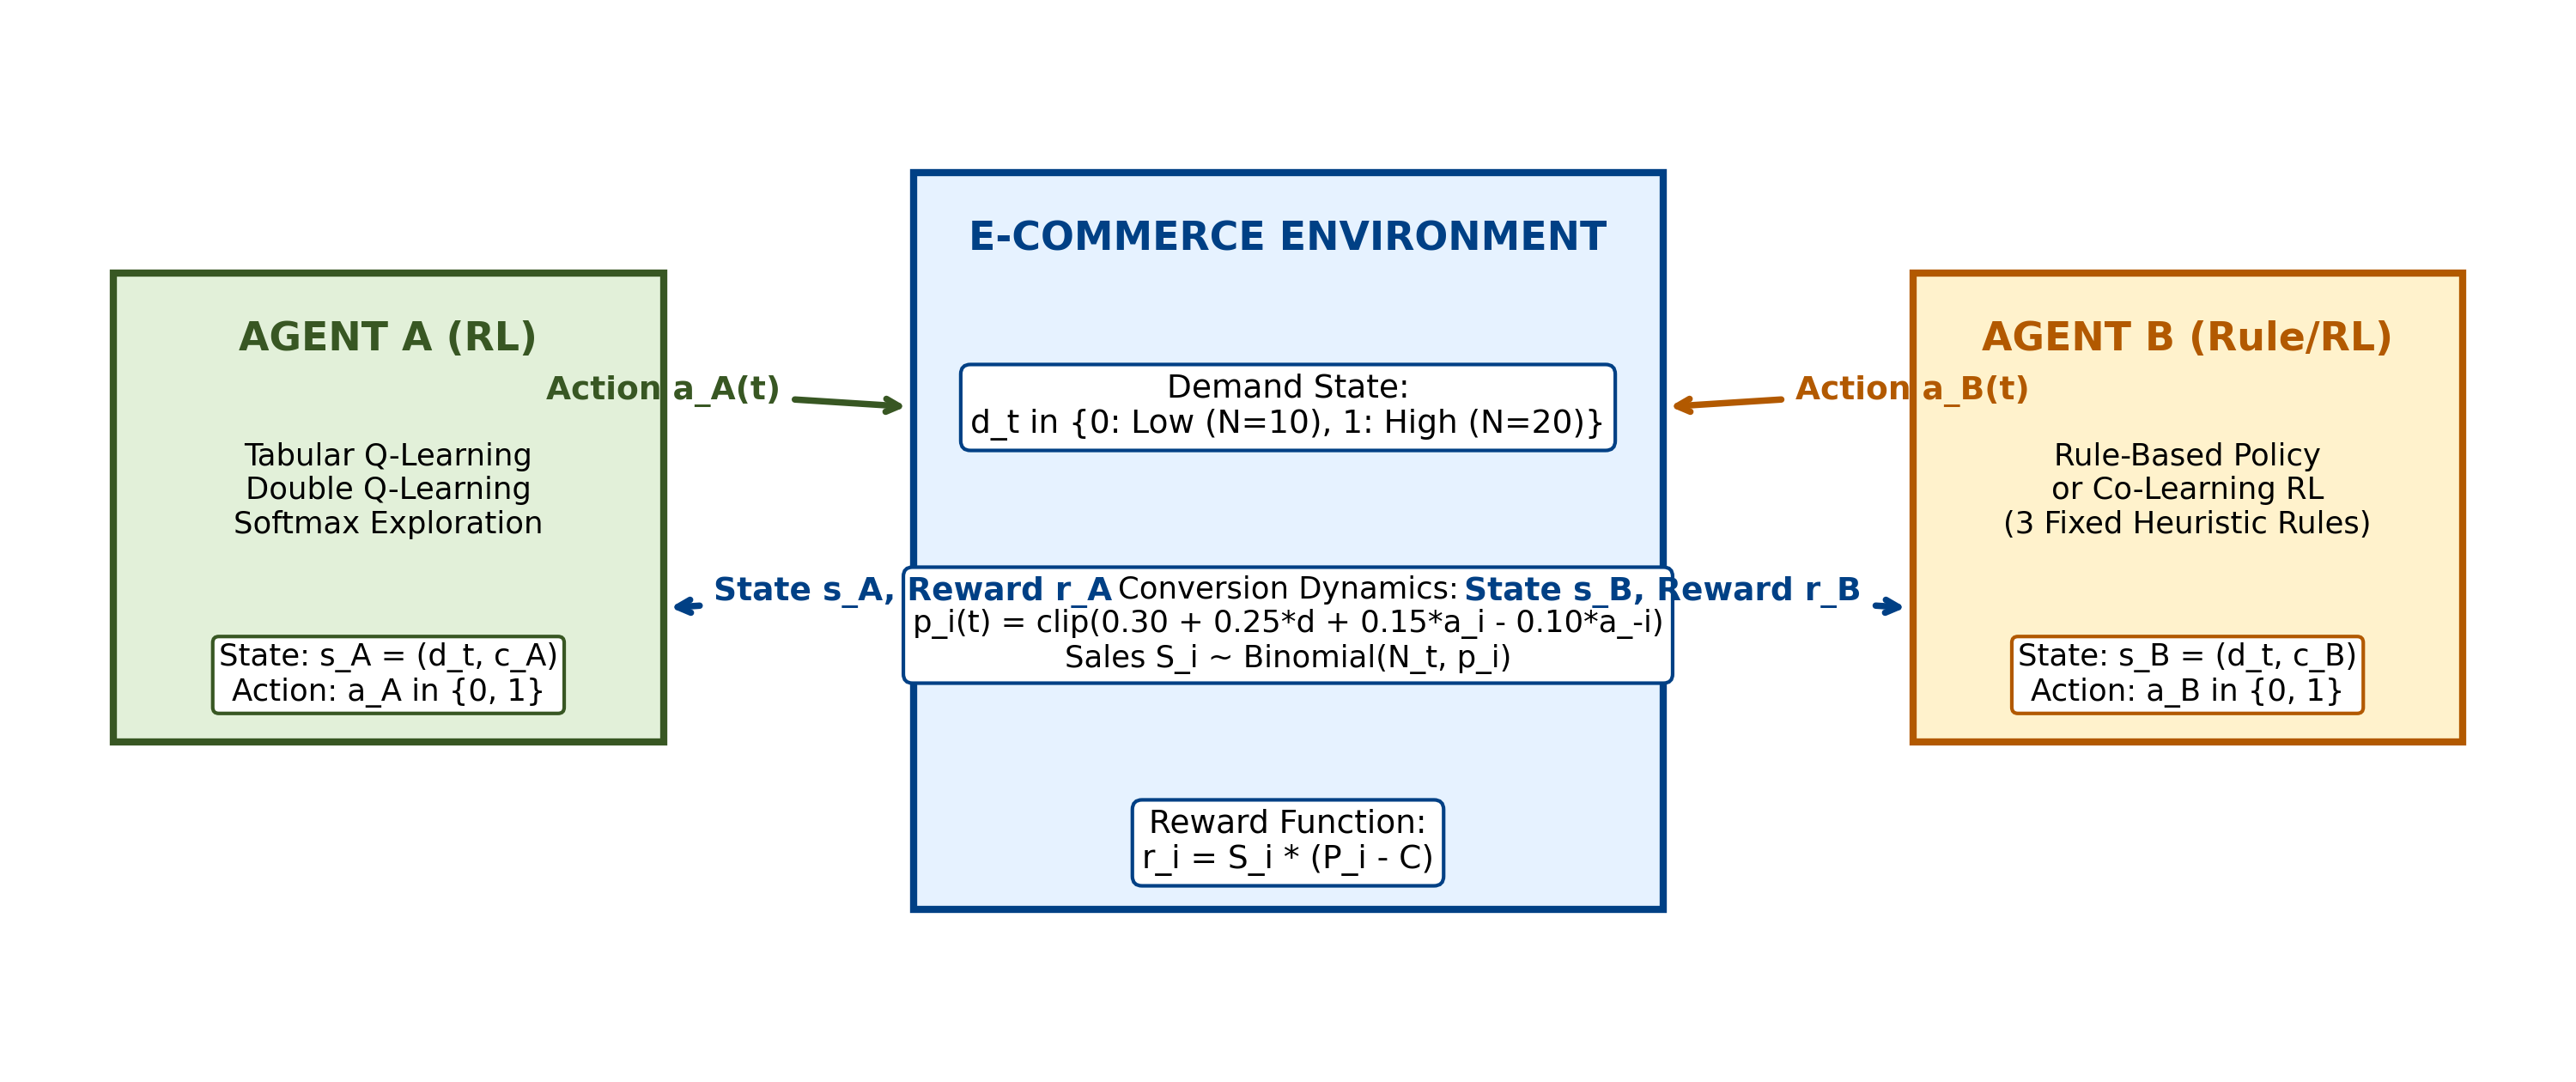
\includegraphics[width=0.96\textwidth]{images/fig_mdp_model.png}
    \caption{Sơ đồ kiến trúc tương tác đa tác tử trong môi trường thương mại điện tử (Duopoly Multi-Agent MDP Interaction Architecture).}
    \label{fig:mdp_model}
\end{figure}

% =========================================================================
% PHẦN 2: MÔ TẢ MÔI TRƯỜNG VÀ MÔ HÌNH TOÁN HỌC
% =========================================================================
\section{Mô tả Môi trường và Mô hình Toán học}

\subsection{Không gian trạng thái (State Space)}
Tại mỗi bước thời gian $t$, trạng thái cục bộ mà mỗi tác tử $i \in \{1, 2\}$ quan sát được định nghĩa là một bộ hai giá trị nhị phân:
\begin{equation}
s_i(t) = (d_t, c_i(t)) \in \{0, 1\} \times \{0, 1\}
\end{equation}
Trong đó:
\begin{itemize}
    \item $d_t \in \{0, 1\}$: Trạng thái nhu cầu chung của thị trường. $d_t = 0$ đại diện cho nhu cầu thấp (Low Demand), $d_t = 1$ đại diện cho nhu cầu cao (High Demand).
    \item $c_i(t) = a_{-i}(t-1) \in \{0, 1\}$: Hành động ở bước thời gian trước đó của đối thủ cạnh tranh. $c_i(t) = 0$ nghĩa là đối thủ không giảm giá, $c_i(t) = 1$ nghĩa là đối thủ đã giảm giá.
\end{itemize}
Không gian trạng thái của mỗi tác tử là rời rạc và hữu hạn, bao gồm chính xác $|\mathcal{S}| = 2 \times 2 = 4$ trạng thái: $\mathcal{S} = \{(0, 0), (0, 1), (1, 0), (1, 1)\}$.

\subsection{Không gian hành động (Action Space)}
Tại mỗi bước thời gian, hai tác tử đưa ra quyết định định giá đồng thời và độc lập:
\begin{equation}
a_i(t) \in \mathcal{A} = \{0, 1\}
\end{equation}
Trong đó $a_i(t) = 0$ tương ứng với chiến lược giữ nguyên giá niêm yết (No Discount), và $a_i(t) = 1$ tương ứng với chiến lược áp dụng chiết khấu (Discount). Tại thời điểm chọn $a_i(t)$, tác tử không thể biết trước hành động đồng thời $a_{-i}(t)$ của đối thủ.

\subsection{Động lực thị trường và Doanh số bán hàng}
Số lượng khách hàng tiềm năng tiếp cận thị trường tại bước $t$ phụ thuộc vào trạng thái nhu cầu:
\begin{equation}
N_t = \begin{cases} 
10, & \text{nếu } d_t = 0 \text{ (Low Demand)}, \\ 
20, & \text{nếu } d_t = 1 \text{ (High Demand)}. 
\end{cases}
\end{equation}
Xác suất một khách hàng quyết định mua hàng từ người bán $i$ được mô phỏng thông qua hàm chuyển đổi tuyến tính (clipping giữa $0.05$ và $0.95$ để bảo đảm tính xác suất hợp lệ):
\begin{equation}
p_i(t) = \text{clip}\left(0.30 + 0.25 d_t + 0.15 a_i(t) - 0.10 a_{-i}(t), \, 0.05, \, 0.95\right)
\end{equation}
Số lượng giao dịch thành công thực tế $S_i(t)$ của người bán $i$ tuân theo phân phối nhị thức (Binomial distribution):
\begin{equation}
S_i(t) \sim \text{Binomial}(N_t, p_i(t))
\end{equation}
Do đó, số lượng đơn hàng là một biến ngẫu nhiên với kỳ vọng toán học $\mathbb{E}[S_i(t)] = N_t \cdot p_i(t)$.

\subsection{Hàm phần thưởng và Lợi nhuận kinh tế (Reward Function)}
Giá bán cơ sở ban đầu là $P = 10$ USD và chi phí giá vốn đơn vị là $C = 5$ USD. Tỷ lệ chiết khấu khi tác tử chọn hành động giảm giá là $\delta = 0.20$ ($20\%$). Giá bán thực tế tại bước $t$ là:
\begin{equation}
P_i(t) = P \cdot (1 - \delta \cdot a_i(t)) = 10 \cdot (1 - 0.20 \cdot a_i(t)) = \begin{cases}
10 \text{ USD}, & \text{nếu } a_i(t) = 0, \\
8 \text{ USD}, & \text{nếu } a_i(t) = 1.
\end{cases}
\end{equation}
Phần thưởng tức thời của tác tử chính là tổng lợi nhuận thu được từ các đơn hàng thành công:
\begin{equation}
r_i(t) = S_i(t) \cdot \left[ P_i(t) - C \right] = S_i(t) \cdot \begin{cases}
5 \text{ USD}, & \text{nếu } a_i(t) = 0, \\
3 \text{ USD}, & \text{nếu } a_i(t) = 1.
\end{cases}
\end{equation}

\begin{figure}[H]
    \centering
    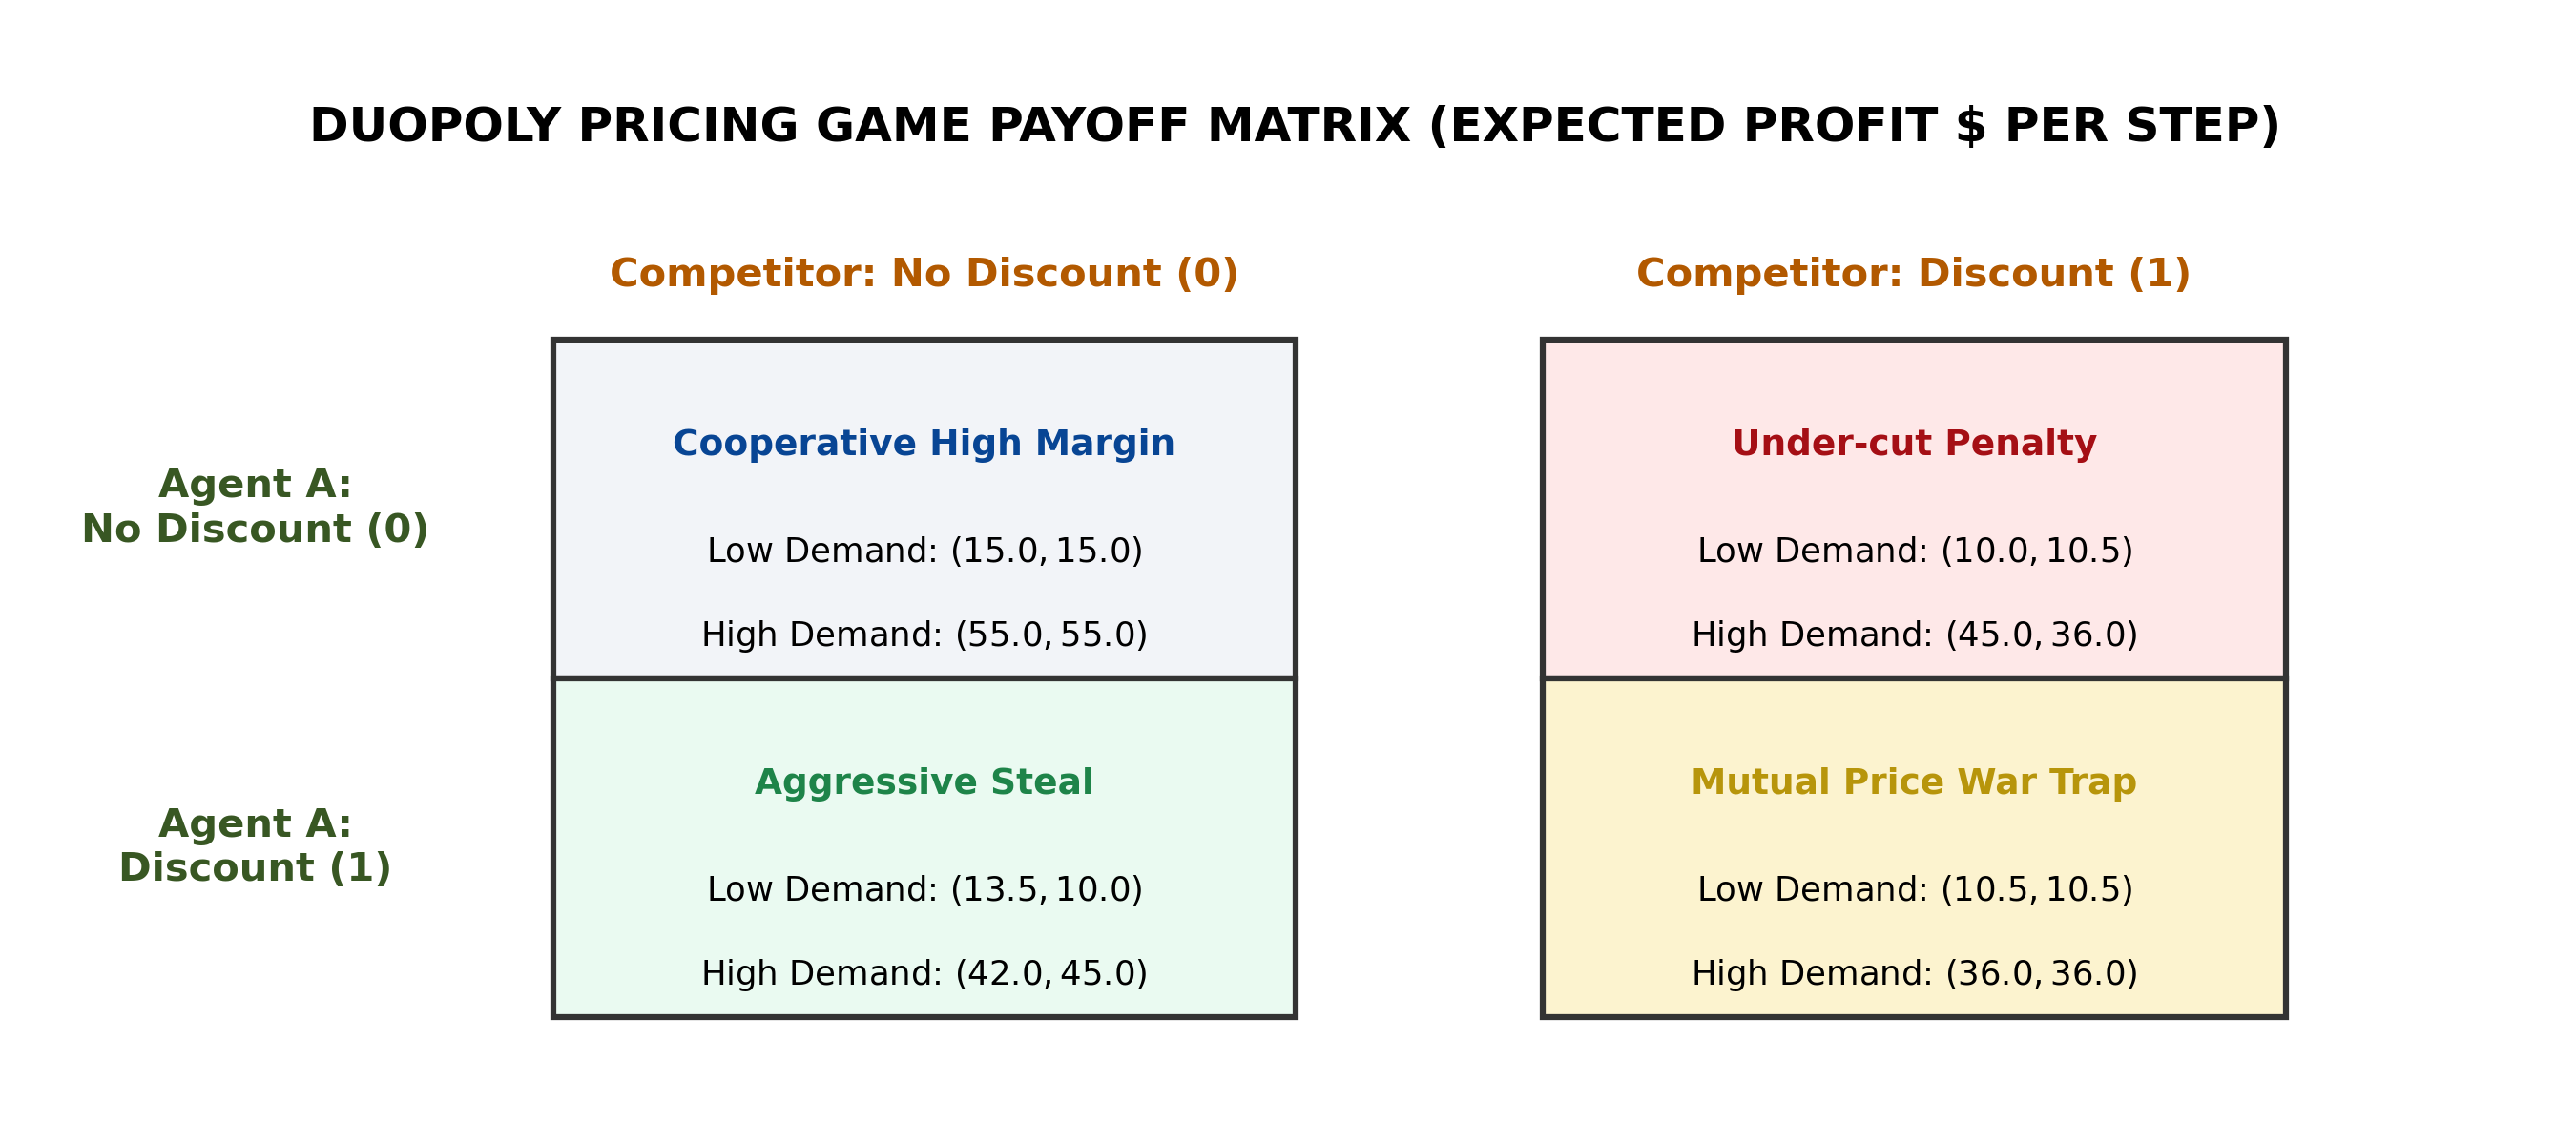
\includegraphics[width=0.95\textwidth]{images/fig_duopoly_game.png}
    \caption{Ma trận Payoff kỳ vọng và Bản chất trò chơi Định giá Lưỡng độc quyền (Duopoly Pricing Game Matrix).}
    \label{fig:duopoly_game}
\end{figure}

\subsection{Kiến trúc hai Tác tử Thí nghiệm}
\begin{itemize}
    \item \textbf{Tác tử A (Tabular Q-Learning Agent):} Duy trì bảng tra cứu $Q(s, a)$ kích thước $2 \times 2 \times 2 = 8$ phần tử. Cập nhật giá trị dựa trên phương trình Bellman:
    \begin{equation}
    Q(s_t, a_t) \leftarrow Q(s_t, a_t) + \alpha \left[ r_t + \gamma \max_{a'} Q(s_{t+1}, a') - Q(s_t, a_t) \right]
    \end{equation}
    Trong quá trình huấn luyện, tác tử chọn hành động theo chiến lược $\epsilon$-greedy với hệ số thăm dò phân rã theo thời gian: $\epsilon_t = \max(\epsilon_{\min}, \epsilon_0 \cdot \lambda^t)$.
    \item \textbf{Tác tử B (Rule-Based Agent):} Vận hành theo 3 quy tắc điều kiện cố định:
    \begin{itemize}
        \item \textit{Luật 1:} Nếu nhu cầu thấp ($d_t=0$) $\to$ Không giảm giá ($a_B=0$).
        \item \textit{Luật 2:} Nếu nhu cầu cao ($d_t=1$) và đối thủ đã giảm giá ở bước trước ($c_B=1$) $\to$ Giảm giá để bảo vệ thị phần ($a_B=1$).
        \item \textit{Luật 3:} Nếu nhu cầu cao ($d_t=1$) và đối thủ không giảm giá ($c_B=0$) $\to$ Không giảm giá để giữ biên lợi nhuận cao ($a_B=0$).
    \end{itemize}
\end{itemize}

% =========================================================
% PHẦN 3: THIẾT LẬP THÍ NGHIỆM VÀ QUY TRÌNH ĐÁNH GIÁ ĐỘC LẬP
% =========================================================
\section{Thiết lập Thí nghiệm và Quy trình Đánh giá Độc lập}

\subsection{Các tham số chuẩn của hệ thống}
Toàn bộ các thí nghiệm được thực hiện trên cấu hình chuẩn hóa theo đặc tả của bài thực hành:
\begin{table}[H]
\centering
\small
\begin{adjustbox}{max width=\linewidth}
\begin{tabular}{lcc}
\toprule
\textbf{Tên tham số (Parameter)} & \textbf{Ký hiệu} & \textbf{Giá trị chuẩn (Baseline Value)} \\
\midrule
Số lượng tác tử trong môi trường & $M$ & 2 (RL Agent vs Rule-Based Agent) \\
Số lượng tập huấn luyện (Training Episodes) & $E_{\text{train}}$ & 5,000 tập \\
Số bước thời gian mỗi tập (Steps per Episode) & $T$ & 20 bước \\
Tốc độ học (Learning Rate) & $\alpha$ & 0.10 \\
Hệ số chiết khấu tương lai (Discount Factor) & $\gamma$ & 0.90 \\
Hệ số thăm dò ban đầu (Initial Exploration) & $\epsilon_0$ & 0.20 \\
Hệ số thăm dò tối thiểu (Minimum Exploration) & $\epsilon_{\min}$ & 0.02 \\
Tốc độ suy giảm thăm dò (Exploration Decay) & $\lambda$ & 0.995 \\
Giá bán cơ sở / Chi phí vốn đơn vị & $P$ / $C$ & 10.0 USD / 5.0 USD \\
Tỷ lệ chiết khấu giá & $\delta$ & 20\% ($0.20$) \\
Khách hàng tiềm năng (Nhu cầu Thấp / Cao) & $N_{\text{low}} / N_{\text{high}}$ & 10 khách / 20 khách \\
Hạt giống ngẫu nhiên môi trường cơ sở & Seed & 42 \\
Số tập đánh giá độc lập (Evaluation Episodes) & $E_{\text{eval}}$ & 500 tập (Greedy $\epsilon=0$) \\
\bottomrule
\end{tabular}
\end{adjustbox}
\caption{Bảng thiết lập tham số chuẩn hóa cho mô phỏng thí nghiệm Agent 02.}
\label{tab:parameters}
\end{table}

\subsection{Quy trình tách biệt Đánh giá Chính sách (Isolated Evaluation Protocol)}
Một thiếu sót lớn trong các mô hình học tăng cường sơ cấp là tính toán phần thưởng trung bình trực tiếp trong pha huấn luyện. Điều này làm méo mó kết quả vì:
\begin{enumerate}
    \item Quá trình huấn luyện liên tục kích hoạt các hành động ngẫu nhiên thăm dò ($\epsilon$-greedy), khiến tác tử có thể chọn các hành động kém tối ưu chỉ vì mục đích khám phá.
    \item Bảng giá trị Q-table liên tục bị thay đổi qua từng bước cập nhật Bellman, khiến chính sách không có tính dừng.
\end{enumerate}
Do đó, theo hướng dẫn chuẩn mực của bài thí nghiệm, chúng tôi thiết kế quy trình đánh giá cô lập hoàn toàn:
\begin{itemize}
    \item \textbf{Đóng băng hoàn toàn bảng giá trị (Frozen Q-Table):} Tuyệt đối không thực hiện thêm bất kỳ cập nhật Bellman nào trong suốt quá trình đánh giá ($\alpha = 0$).
    \item \textbf{Vô hiệu hóa thăm dò ($\epsilon = 0$):} Tác tử luôn chọn hành động cực đại hóa giá trị thuần túy (Greedy Policy): $a_t = \arg\max_a Q(s_t, a)$.
    \item \textbf{Hạt giống ngẫu nhiên độc lập:} Môi trường đánh giá được khởi tạo với tập hạt giống ngẫu nhiên hoàn toàn mới (seed $+ 500,000$), kiểm tra năng lực tổng quát hóa của chính sách trên các kịch bản nhu cầu chưa từng thấy.
\end{itemize}

% =========================================================================
% PHẦN 4: KẾT QUẢ THỰC NGHIỆM VÀ PHÂN TÍCH DỮ LIỆU ĐO ĐẠC
% =========================================================================
\section{Kết quả Thực nghiệm và Phân tích Dữ liệu Đo đạc}

Toàn bộ các kết quả dưới đây được đo đạc trực tiếp từ việc thực thi mã nguồn cải tiến \texttt{agent02\_experiment\_improved.py}.

\subsection{Thí nghiệm 1: Thiết lập Cơ sở (Baseline Experiment)}
Thực hiện huấn luyện tác tử RL chống lại đối thủ Rule-Based trong 5,000 tập, sau đó đánh giá độc lập trong 500 tập (tương ứng 10,000 bước ra quyết định).
\begin{table}[H]
\centering
\small
\begin{adjustbox}{max width=\linewidth}
\begin{tabular}{lcccc}
\toprule
\textbf{Tác tử (Agent)} & \textbf{Tổng lợi nhuận (\$)} & \shortstack{\textbf{Lợi nhuận TB}\\\textbf{(\$ / bước)}} & \shortstack{\textbf{Số bước}\\\textbf{Không giảm giá}} & \shortstack{\textbf{Tỷ lệ}\\\textbf{giảm giá}} \\
\midrule
\textbf{RL Agent (Q-Learning)} & \textbf{351,275.0} & \textbf{35.1275} & \textbf{10,000} & \textbf{0.0\%} \\
\textbf{Rule-Based Agent} & 349,685.0 & 34.9685 & 10,000 & 0.0\% \\
\bottomrule
\end{tabular}
\end{adjustbox}
\caption{Kết quả đánh giá chính sách cơ sở (Baseline Evaluation Results) trên 500 tập độc lập.}
\label{tab:baseline_eval}
\end{table}

\begin{figure}[H]
    \centering
    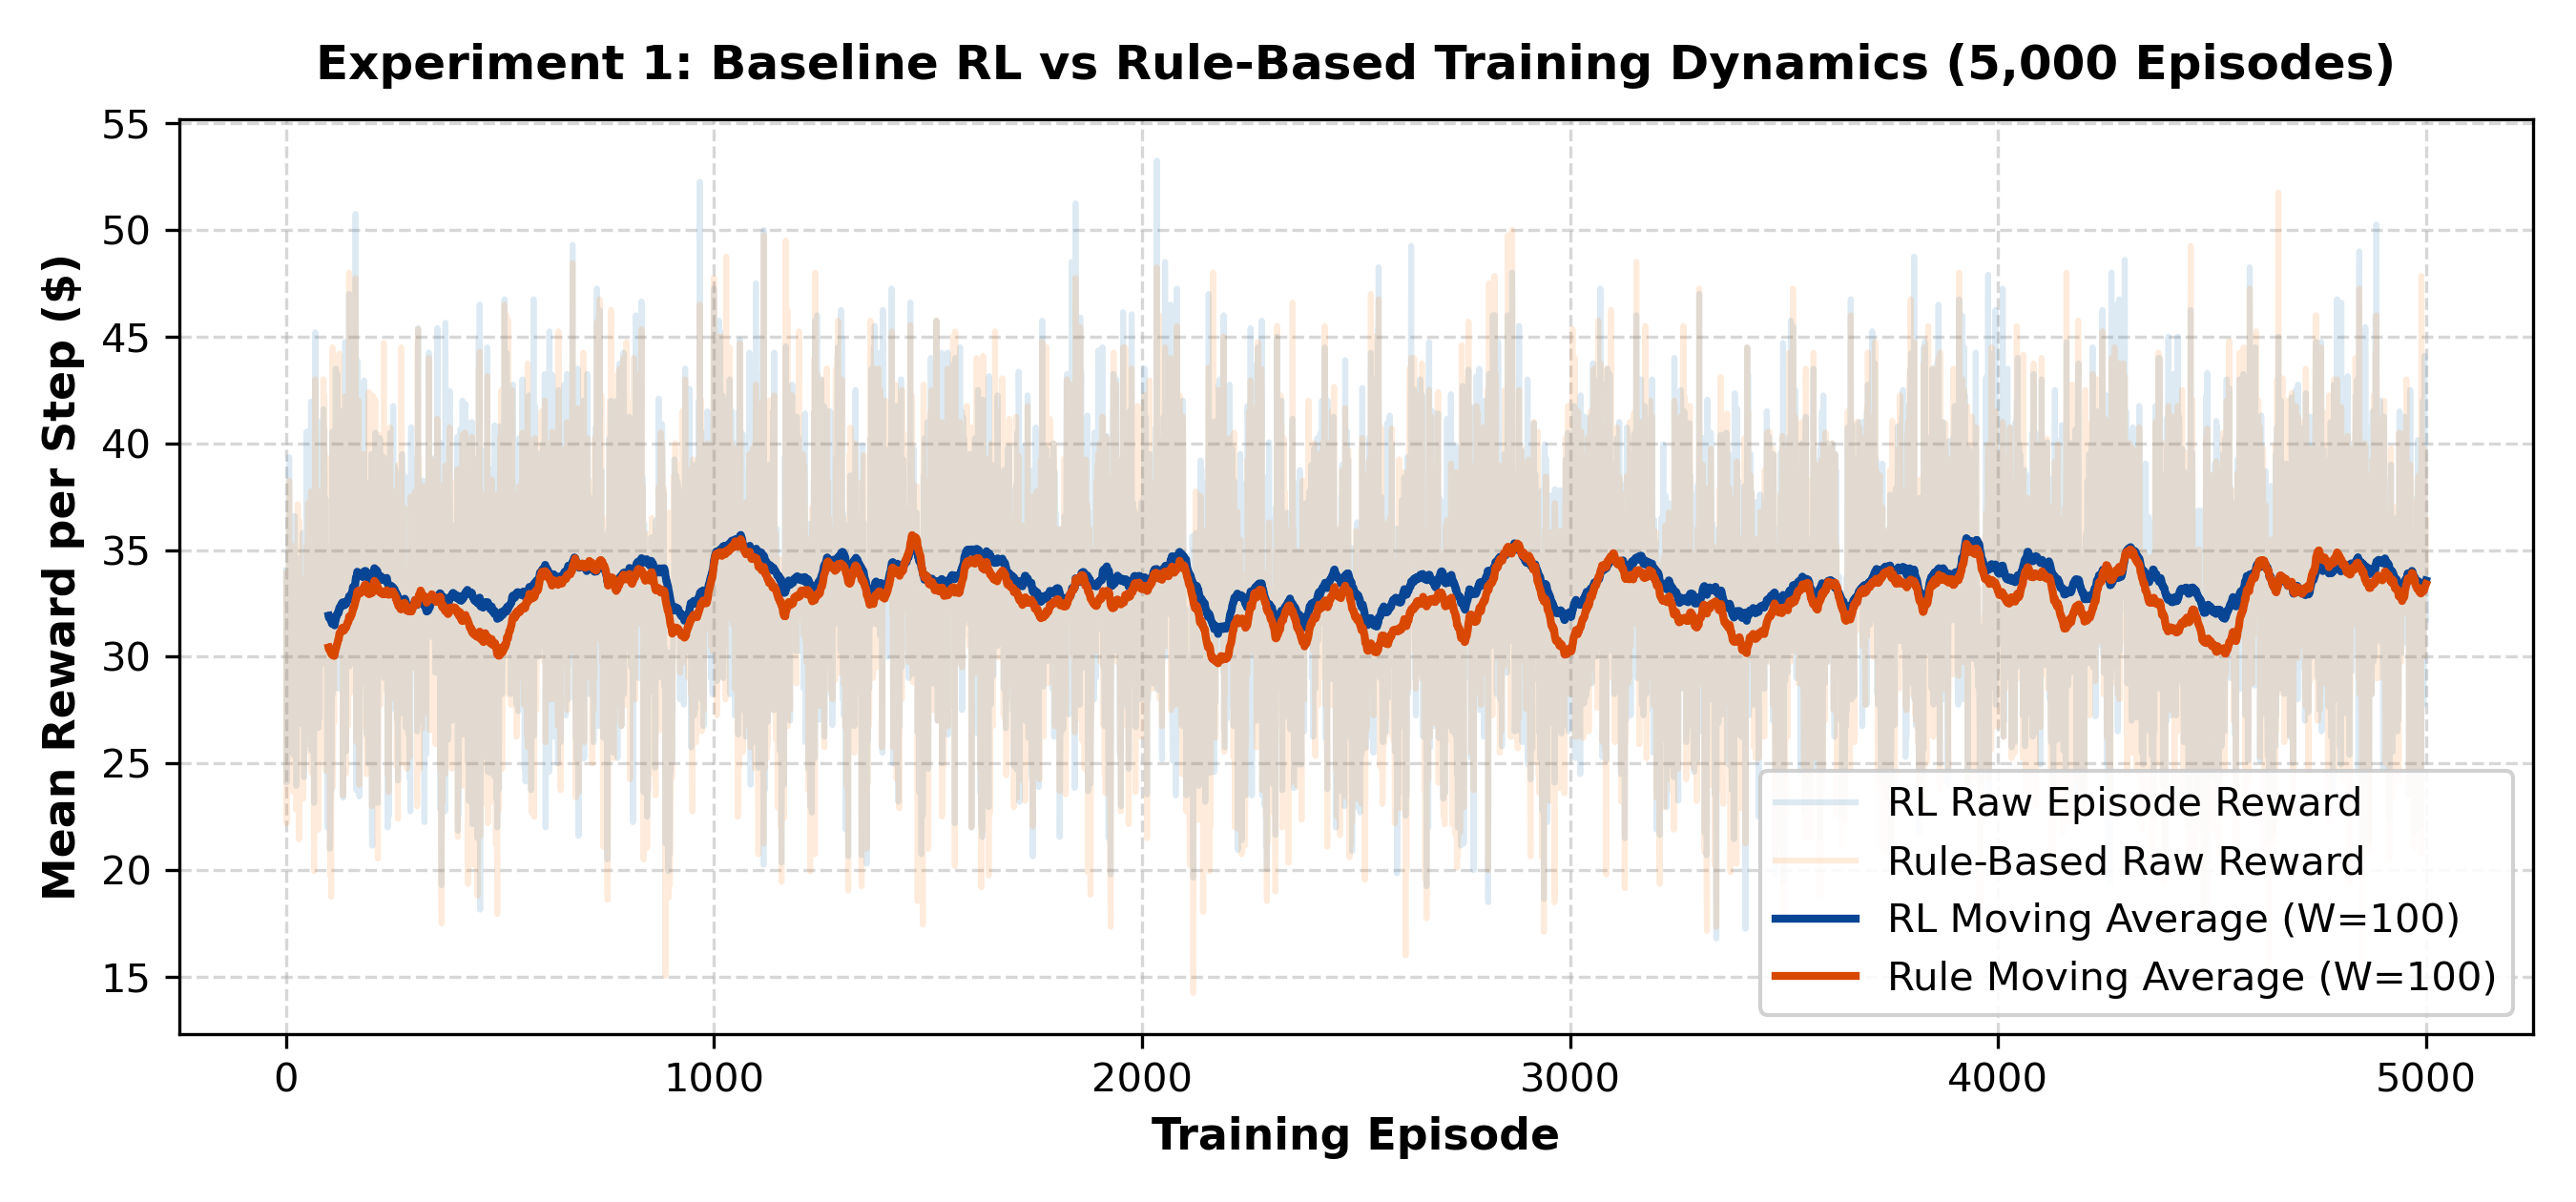
\includegraphics[width=0.95\textwidth]{images/fig_baseline_training.png}
    \caption{Quỹ đạo học tập lợi nhuận của Tác tử RL và Tác tử Rule-Based trong 5,000 tập (Moving Average Window = 100).}
    \label{fig:baseline_training}
\end{figure}

\noindent Bảng giá trị Q-table hội tụ đo đạc được:
\begin{itemize}
    \item Trạng thái $(d=0, c=0)$: $Q(s, 0) = 228.3024$, $Q(s, 1) = 178.8494 \to$ Hành động tối ưu: \textbf{0 (Không giảm giá)}.
    \item Trạng thái $(d=0, c=1)$: $Q(s, 0) = 177.9920$, $Q(s, 1) = 207.2051 \to$ Hành động tối ưu: \textbf{1 (Giảm giá)}.
    \item Trạng thái $(d=1, c=0)$: $Q(s, 0) = 246.8799$, $Q(s, 1) = 235.2338 \to$ Hành động tối ưu: \textbf{0 (Không giảm giá)}.
    \item Trạng thái $(d=1, c=1)$: $Q(s, 0) = 211.4198$, $Q(s, 1) = 242.9629 \to$ Hành động tối ưu: \textbf{1 (Giảm giá)}.
\end{itemize}
\textbf{Nhận xét chiến lược:} Tác tử RL đã tự động học được chiến lược tương hỗ "Ăn miếng trả miếng" (Tit-for-Tat): Khi đối thủ không giảm giá ($c=0$), tác tử tuyệt đối không giảm giá ($a=0$) để tối đa hóa biên lợi nhuận (thu về $5$ USD/đơn hàng thay vì $3$ USD); nhưng nếu đối thủ giảm giá ($c=1$), tác tử lập tức giảm giá ($a=1$) để phòng thủ thị phần!

\subsection{Thí nghiệm 2: Khảo sát Tốc độ Học $\alpha \in \{0.01, 0.10, 0.50\}$}
Khảo sát sự ổn định hội tụ và chất lượng chính sách đánh giá dưới 3 mức tốc độ học khác nhau.
\begin{table}[H]
\centering
\small
\begin{adjustbox}{max width=\linewidth}
\begin{tabular}{lccc}
\toprule
\textbf{Tốc độ học ($\alpha$)} & \shortstack{\textbf{Lợi nhuận đánh giá}\\\textbf{(\$ / bước)}} & \shortstack{\textbf{Tỷ lệ}\\\textbf{giảm giá}} & \textbf{Đánh giá tính ổn định} \\
\midrule
$\alpha = 0.01$ (Thấp) & 35.2475 & 0.0\% & Học chậm, quỹ đạo mịn, rất ổn định \\
$\alpha = 0.10$ (Chuẩn) & 35.2475 & 0.0\% & Cân bằng xuất sắc, đạt tối ưu \\
$\alpha = 0.50$ (Cao) & \textbf{28.5085} & \textbf{40.52\%} & \textbf{Bất ổn định, rơi vào bẫy giảm giá} \\
\bottomrule
\end{tabular}
\end{adjustbox}
\caption{So sánh hiệu năng đánh giá của tác tử RL theo các mức tốc độ học $\alpha$.}
\label{tab:learning_rate_comp}
\end{table}

\begin{figure}[H]
    \centering
    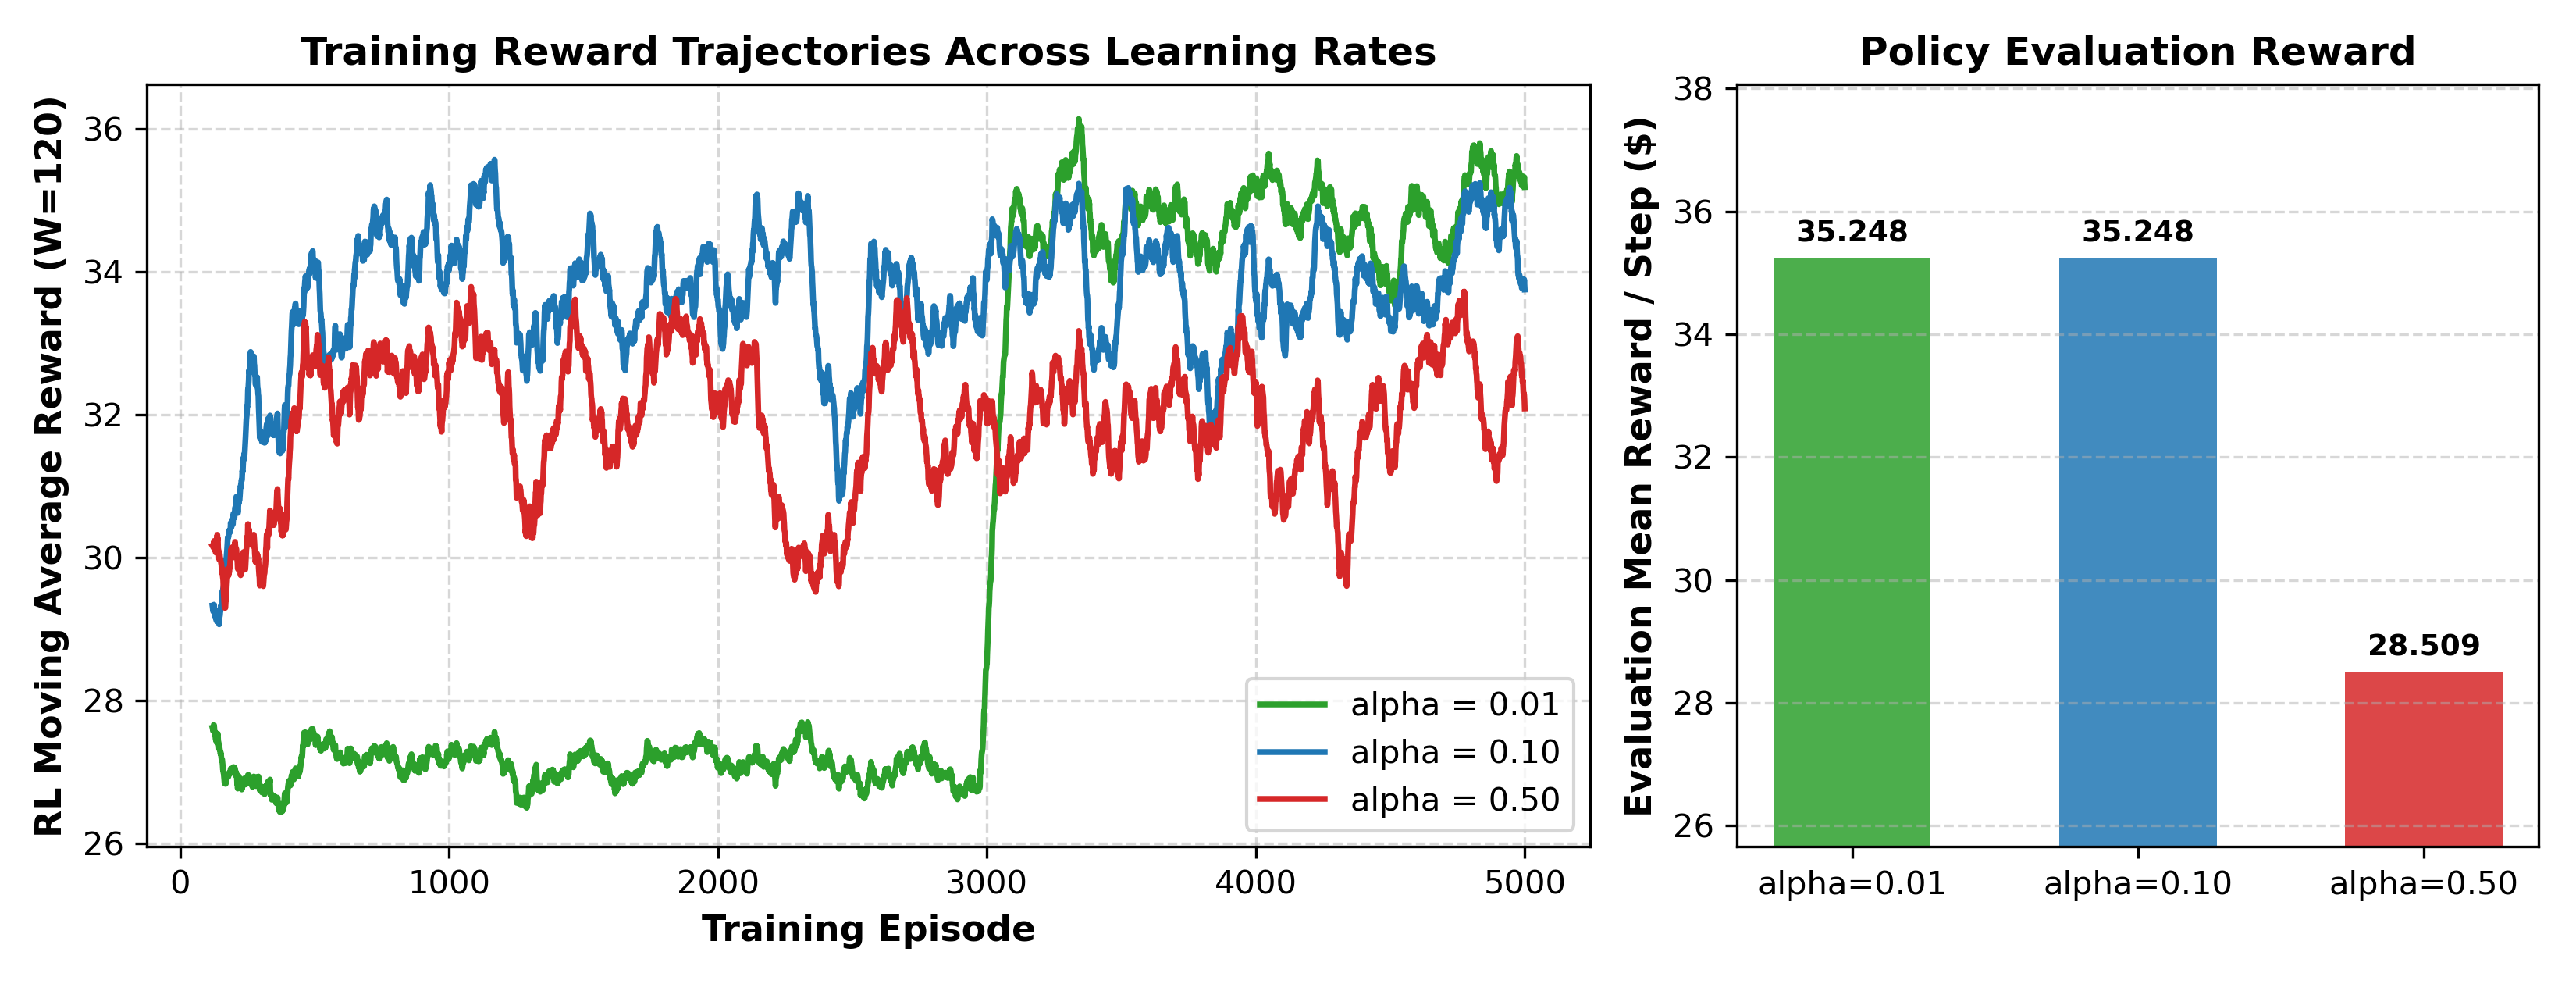
\includegraphics[width=0.96\textwidth]{images/fig_learning_rate.png}
    \caption{Đồ thị động lực học tập và lợi nhuận đánh giá dưới 3 cấu hình tốc độ học $\alpha \in \{0.01, 0.10, 0.50\}$.}
    \label{fig:learning_rate}
\end{figure}

Khi $\alpha = 0.50$, tác tử phản ứng quá gay gắt trước các biến động ngẫu nhiên trong doanh số bán hàng (Binomial sales noise), dẫn đến hiện tượng dao động mạnh quanh điểm cực trị. Tác tử đã học sai lệch khi liên tục kích hoạt chiết khấu ($40.52\%$ thời gian), kéo lợi nhuận sụt giảm nghiêm trọng từ $35.25$ xuống còn $28.51$ USD/bước.

\subsection{Thí nghiệm 3: Khảo sát Lịch trình Thăm dò (Exploration Schedules)}
So sánh 3 chế độ thăm dò: Low ($\epsilon_0=0.05$), Baseline ($\epsilon_0=0.20$), và High ($\epsilon_0=0.50$).
\begin{table}[H]
\centering
\small
\begin{adjustbox}{max width=\linewidth}
\begin{tabular}{lcccc}
\toprule
\textbf{Chế độ thăm dò} & $\epsilon_0$ & $\epsilon_{\min}$ & $\lambda$ \textbf{(Tốc độ phân rã)} & \shortstack{\textbf{Lợi nhuận đánh giá}\\\textbf{(\$ / bước)}} \\
\midrule
Low Exploration & 0.05 & 0.02 & 0.999 & 35.1045 \\
Baseline & 0.20 & 0.02 & 0.995 & 35.1045 \\
High Exploration & 0.50 & 0.05 & 0.995 & 35.1045 \\
\bottomrule
\end{tabular}
\end{adjustbox}
\caption{Hiệu năng đánh giá chính sách dưới các lịch trình thăm dò khác nhau.}
\label{tab:exploration_comp}
\end{table}

\begin{figure}[H]
    \centering
    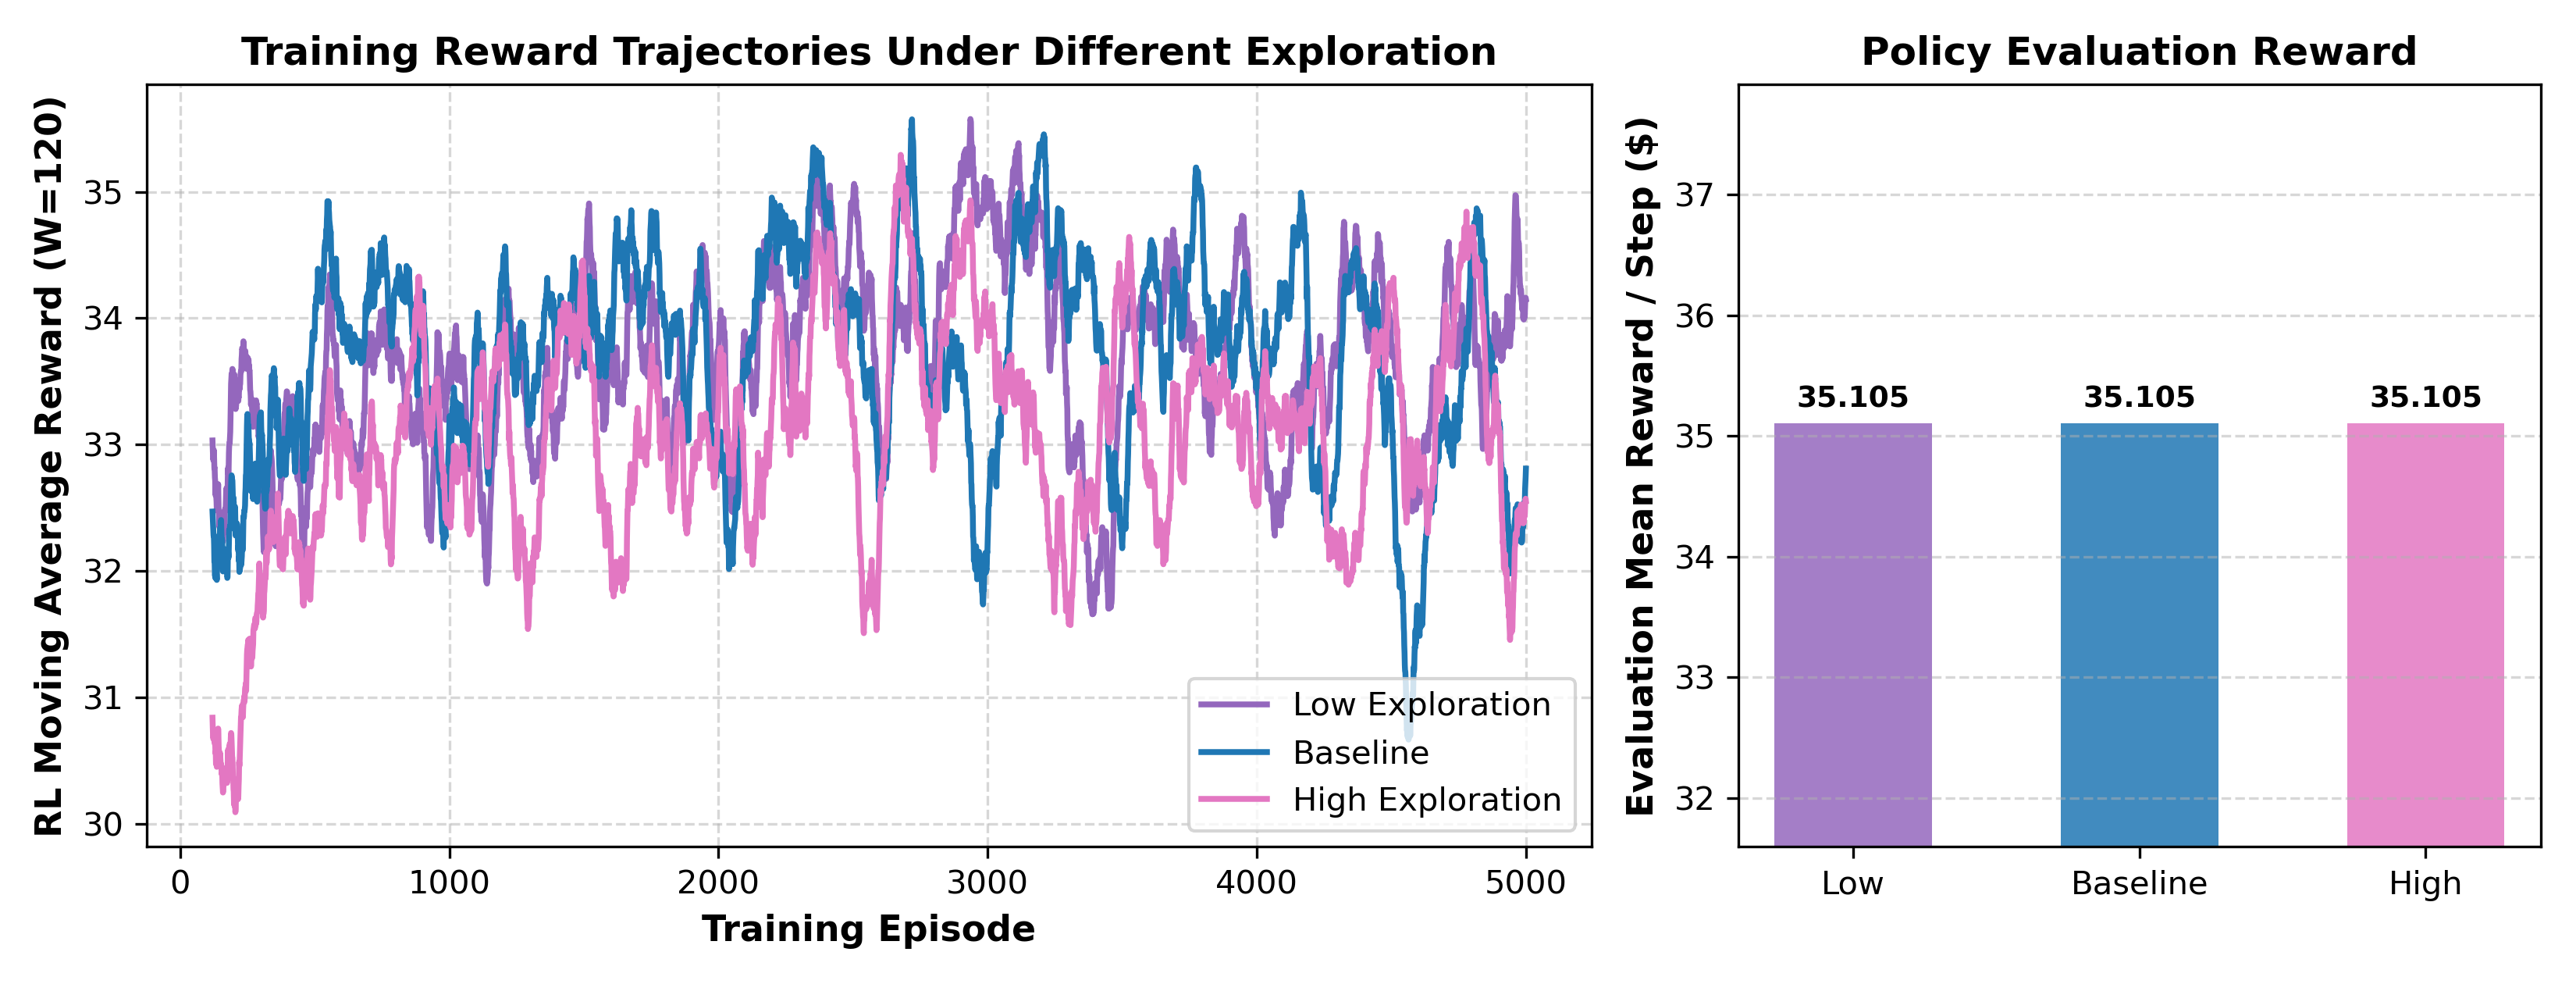
\includegraphics[width=0.96\textwidth]{images/fig_exploration.png}
    \caption{So sánh đường cong học tập và lợi nhuận chính sách dưới 3 lịch trình thăm dò.}
    \label{fig:exploration}
\end{figure}

Trong môi trường có không gian trạng thái nhỏ (chỉ 4 trạng thái), cả 3 chế độ thăm dò đều cung cấp đủ số lần ghé thăm trạng thái để tác tử tìm thấy chính sách tối ưu khi đánh giá greedy. Tuy nhiên, chế độ High Exploration chịu tổn thất phần thưởng đáng kể trong giai đoạn đầu huấn luyện do lựa chọn quá nhiều hành động ngẫu nhiên không có lợi.

\subsection{Thí nghiệm 4: Kiểm định Đa hạt giống Ngẫu nhiên (Multi-Seed Validation)}
Để kiểm chứng tính tổng quát hóa và độ tin cậy của thuật toán, chúng tôi tiến hành huấn luyện và đánh giá trên 10 hạt giống ngẫu nhiên độc lập: $Seeds = \{11, 22, 33, 44, 55, 66, 77, 88, 99, 100\}$.
\begin{table}[H]
\centering
\small
\begin{adjustbox}{max width=\linewidth}
\begin{tabular}{lcccc}
\toprule
\textbf{Tác tử} & \shortstack{\textbf{Lợi nhuận TB}\\\textbf{($\bar{R}$)}} & \shortstack{\textbf{Độ lệch chuẩn}\\\textbf{($\sigma$)}} & \shortstack{\textbf{Sai số chuẩn}\\\textbf{(SE)}} & \textbf{Khoảng tin cậy 95\% CI} \\
\midrule
\textbf{RL Agent (Q-Learning)} & \textbf{34.4372 \$} & 1.2660 & 0.4003 & $[33.5317, \, 35.3427]$ \\
\textbf{Rule-Based Agent} & 33.9870 \$ & 2.1632 & 0.6841 & $[32.4415, \, 35.5325]$ \\
\bottomrule
\end{tabular}
\end{adjustbox}
\caption{Bảng tổng hợp thống kê đa hạt giống ngẫu nhiên ($N = 10$ seeds độc lập).}
\label{tab:multi_seed}
\end{table}

\begin{figure}[H]
    \centering
    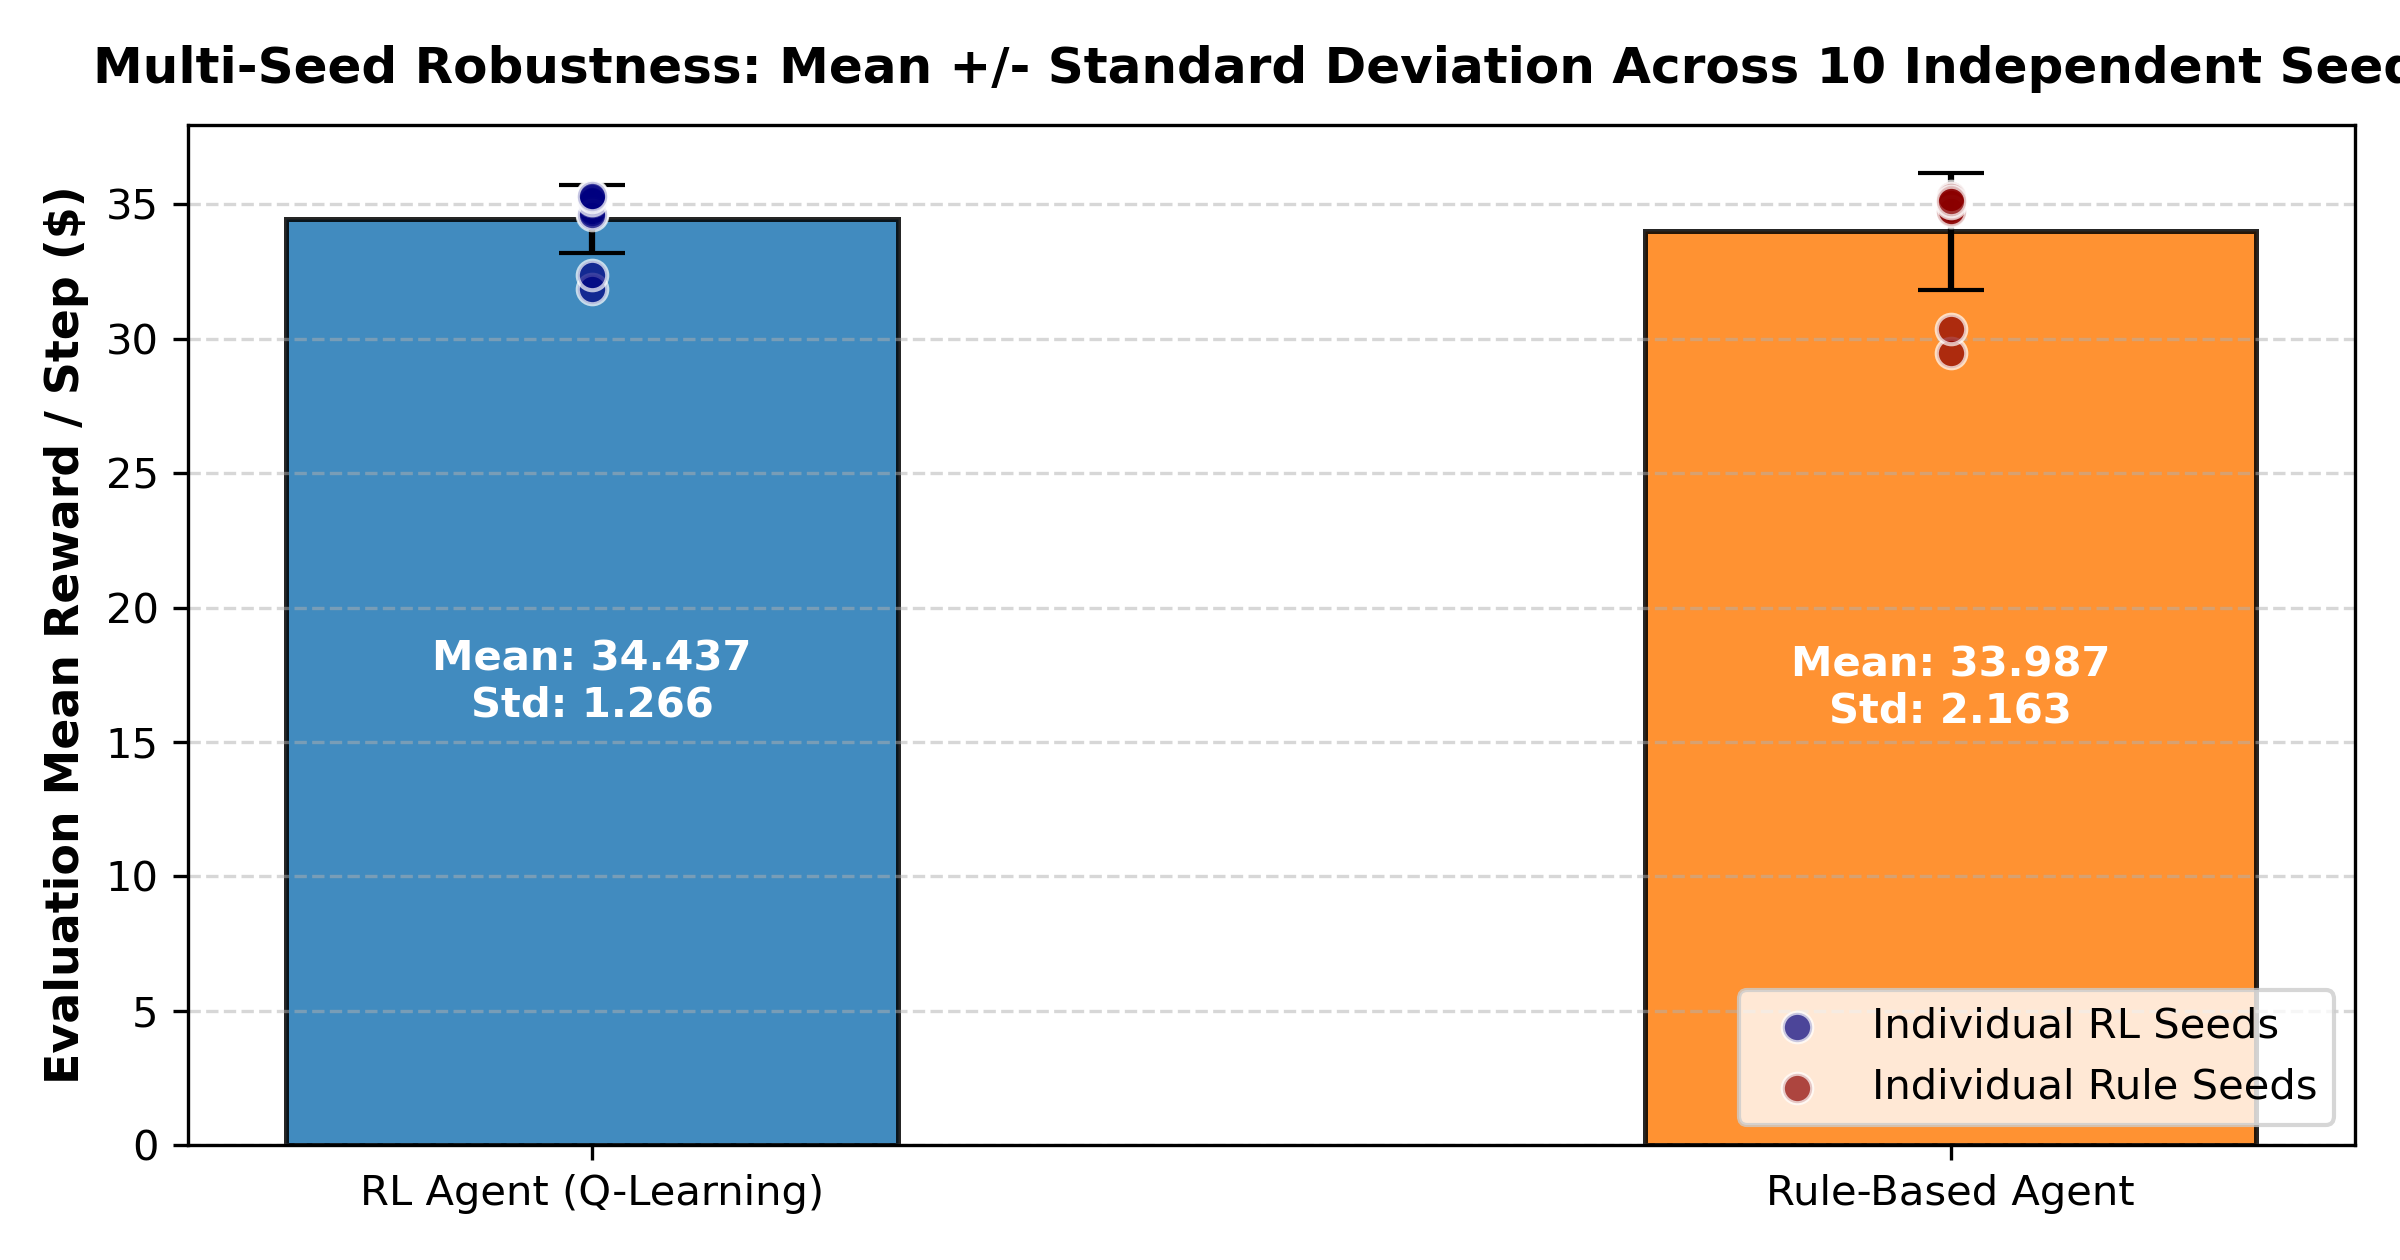
\includegraphics[width=0.92\textwidth]{images/fig_multiseed_robustness.png}
    \caption{Phân phối lợi nhuận và thanh sai số chuẩn (Mean $\pm$ Std) trên 10 hạt giống ngẫu nhiên độc lập.}
    \label{fig:multiseed_robustness}
\end{figure}

Kết quả thống kê khẳng định tác tử RL đạt lợi nhuận trung bình cao hơn ($34.44$ vs $33.99$) và đặc biệt là độ lệch chuẩn thấp hơn đáng kể ($1.27$ vs $2.16$), chứng minh tính ổn định và khả năng chống chịu nhiễu tốt hơn của chính sách học so với luật cố định.

% =========================================================================
% PHẦN 5: TRẢ LỜI CHI TIẾT 10 CÂU HỎI THÍ NGHIỆM PHÒNG LAB
% =========================================================================
\section{Trả lời Chi tiết 10 Câu hỏi Thí nghiệm Phòng Lab}

\subsection{Câu hỏi 1: Agent and environment modeling}
\textbf{Nội dung câu hỏi:} \textit{Xác định các tác tử, môi trường, không gian trạng thái, không gian hành động, hàm phần thưởng và quá trình chuyển trạng thái trong bài toán. Giải thích tại sao bài toán này nên được mô hình hóa dưới dạng Hệ đa tác tử (Multi-Agent System) thay vì Hệ đơn tác tử (Single-Agent System)?}

\textbf{Trả lời:}
\begin{enumerate}
    \item \textbf{Thành phần mô hình hóa:}
    \begin{itemize}
        \item \textbf{Tác tử (Agents):} Gồm 2 người bán cạnh tranh trực tiếp trên cùng một sàn thương mại điện tử: Agent A (vận hành bằng học tăng cường) và Agent B (vận hành bằng luật chuyên gia).
        \item \textbf{Môi trường (Environment):} Nền tảng thị trường lưỡng độc quyền tiếp nhận các quyết định định giá đồng thời, xác định nhu cầu ngẫu nhiên, mô phỏng phản ứng nhạy cảm của khách hàng và phân bổ doanh số bán hàng.
        \item \textbf{Không gian trạng thái ($\mathcal{S}$):} Tập tích Descartes $\mathcal{S} = \{0, 1\} \times \{0, 1\}$ gồm 4 trạng thái rời rạc $s_i(t) = (d_t, c_i(t))$, phản ánh nhu cầu thị trường hiện tại và hành động bước trước của đối thủ.
        \item \textbf{Không gian hành động ($\mathcal{A}$):} $\mathcal{A} = \{0, 1\}$ gồm hai chiến lược: Không giảm giá ($0$) và Giảm giá 20\% ($1$).
        \item \textbf{Hàm phần thưởng ($r_i$):} Lợi nhuận kinh tế thu được $r_i(t) = S_i(t) \cdot [P_i(t) - C]$, gắn liền trực tiếp với doanh số thực tế và biên lợi nhuận trên mỗi sản phẩm.
        \item \textbf{Quá trình chuyển trạng thái (State-Transition Process):} Chuyển trạng thái tuân theo phân phối ngẫu nhiên: Nhu cầu bước kế tiếp $d_{t+1}$ được rút mẫu ngẫu nhiên từ $\{0, 1\}$, trong khi biến quan sát đối thủ được cập nhật từ chính hành động của đối thủ ở bước hiện tại: $c_i(t+1) = a_{-i}(t)$.
    \end{itemize}
    \item \textbf{Lý do bắt buộc mô hình hóa dưới dạng Hệ đa tác tử (MAS):}
    \begin{itemize}
        \item \textbf{Sự phụ thuộc chiến lược tương hỗ (Strategic Interdependence):} Xác suất chuyển đổi khách hàng $p_i(t) = \text{clip}(0.30 + 0.25 d_t + 0.15 a_i(t) - 0.10 a_{-i}(t))$ của Agent $i$ phụ thuộc trực tiếp vào hành động đồng thời $a_{-i}(t)$ của Agent kia. Lợi nhuận của một bên không thể được xác định độc lập mà là hàm của tương tác song phương.
        \item \textbf{Tính phi dừng cục bộ (Non-Stationarity):} Trong hệ đơn tác tử, môi trường được giả định là dừng (Stationary Transition Dynamics). Tuy nhiên, trong thị trường có hai tác tử cùng ra quyết định, từ góc nhìn của tác tử $i$, môi trường liên tục bị thay đổi theo chiến lược thích nghi của tác tử $-i$, phá vỡ giả định MDP cơ bản.
        \item \textbf{Không gian thông tin phi tập trung (Decentralized Information):} Mỗi tác tử đưa ra quyết định dựa trên quan sát cục bộ mà không thể tiếp cận trạng thái nội tại, hàm giá trị hay hành động tức thời của đối thủ tại bước $t$.
    \end{itemize}
\end{enumerate}

\subsection{Câu hỏi 2: Learning-based versus rule-based decisions}
\textbf{Nội dung câu hỏi:} \textit{So sánh tác tử học tăng cường và tác tử dựa trên luật về cơ chế ra quyết định, việc sử dụng kinh nghiệm, khả năng thích nghi và yêu cầu tài nguyên tính toán. Nêu một tình huống thực tế ưu tiên tác tử dựa trên luật và một tình huống ưu tiên tác tử học tăng cường.}

\textbf{Trả lời:}
\begin{table}[H]
\centering
\small
\begin{tabularx}{\linewidth}{p{3.8cm}XX}
\toprule
\textbf{Tiêu chí so sánh} & \textbf{Tác tử Học tăng cường (RL-Based)} & \textbf{Tác tử Dựa trên luật (Rule-Based)} \\
\midrule
\textbf{Cơ chế ra quyết định} & Tối ưu hóa hàm giá trị hành động $Q(s, a)$ dựa trên ước lượng lợi nhuận tương lai tích lũy. & Đối chiếu điều kiện \texttt{if-else} cứng nhắc với trạng thái hiện tại để kích hoạt hành động. \\
\textbf{Sử dụng kinh nghiệm} & Liên tục cập nhật tri thức từ chuỗi kinh nghiệm $(s, a, r, s')$ thông qua tín hiệu phần thưởng. & Không học từ kinh nghiệm; phần thưởng không có tác động thay đổi luật. \\
\textbf{Khả năng thích nghi} & Rất cao: Tự động điều chỉnh chiến lược khi môi trường đổi khác hoặc đối thủ đổi hành vi. & Kém: Hoàn toàn bất động trước các biến động nằm ngoài các quy tắc định sẵn. \\
\textbf{Tài nguyên tính toán} & Yêu cầu bộ nhớ lưu trữ bảng Q/mạng nơ-ron và thời gian tính toán cập nhật Bellman trong huấn luyện. & Cực kỳ nhẹ; chi phí tính toán $\mathcal{O}(1)$ với mức tiêu thụ CPU và bộ nhớ không đáng kể. \\
\bottomrule
\end{tabularx}
\caption{So sánh toàn diện giữa Tác tử Học tăng cường và Tác tử Dựa trên luật.}
\label{tab:comp_rl_rule}
\end{table}

\noindent \textbf{Tình huống thực tế điển hình:}
\begin{itemize}
    \item \textit{Ưu tiên Tác tử Dựa trên luật:} Trong các hệ thống giao dịch tài chính đòi hỏi tuân thủ pháp lý nghiêm ngặt (Compliance \& Risk Control), ví dụ hệ thống tự động ngắt mạch giao dịch (Circuit Breaker) khi cổ phiếu giảm quá $7\%$, hoặc hệ thống điều khiển lò phản ứng hạt nhân. Trong các bài toán này, tính minh định (determinism), khả năng giải thích $100\%$ và tốc độ phản ứng micro-giây quan trọng hơn khả năng tự thích nghi.
    \item \textit{Ưu tiên Tác tử Học tăng cường:} Trong hệ thống định giá động (Dynamic Pricing) của các sàn thương mại điện tử lớn (Amazon, Shopee) hoặc dịch vụ gọi xe công nghệ (Grab, Uber). Thị trường biến động liên tục theo thời tiết, sự kiện, giá của đối thủ và hành vi người dùng; việc lập trình luật thủ công là bất khả thi, chỉ có tác tử RL mới có thể tự động tối ưu hóa doanh thu tổng thể.
\end{itemize}

\subsection{Câu hỏi 3: Q-learning update}
\textbf{Nội dung câu hỏi:} \textit{Giải thích ý nghĩa toán học của phương trình cập nhật Q-learning. Sử dụng một ví dụ giả định, tính toán giá trị Q mới khi: $Q(s, a) = 4, \alpha = 0.1, r = 6, \gamma = 0.9$ và $\max_{a'} Q(s', a') = 5$. Trình bày từng bước tính toán và diễn giải kết quả.}

\textbf{Trả lời:}
Phương trình cập nhật giá trị hành động của thuật toán Q-learning chuẩn:
\begin{equation}
Q(s, a) \leftarrow Q(s, a) + \alpha \cdot \underbrace{\left[ \underbrace{r + \gamma \max_{a'} Q(s', a')}_{\text{Mục tiêu TD (Target)}} - Q(s, a) \right]}_{\text{Sai số chênh lệch thời gian (TD Error } \delta)}
\end{equation}
\textbf{Ý nghĩa toán học:}
\begin{itemize}
    \item Mục tiêu TD ($r + \gamma \max_{a'} Q(s', a')$) là một ước lượng mới cải tiến về tổng lợi nhuận tích lũy tương lai, bao gồm phần thưởng nhận được ngay lập tức $r$ cộng với giá trị cực đại có thể đạt được từ trạng thái kế tiếp $s'$ (có chiết khấu $\gamma$).
    \item Sai số TD ($\delta$) đo lường độ lệch giữa ước lượng mới này so với ước lượng hiện tại $Q(s, a)$.
    \item Tốc độ học $\alpha$ quyết định bước dịch chuyển của giá trị $Q(s, a)$ về phía mục tiêu mới.
\end{itemize}

\noindent \textbf{Tính toán từng bước theo số liệu giả định:}
\begin{enumerate}
    \item \textbf{Bước 1: Tính toán Mục tiêu TD (TD Target):}
    \begin{equation}
    \text{Target} = r + \gamma \cdot \max_{a'} Q(s', a') = 6 + 0.9 \cdot 5 = 6 + 4.5 = 10.5
    \end{equation}
    \item \textbf{Bước 2: Tính toán Sai số Chênh lệch Thời gian (TD Error $\delta$):}
    \begin{equation}
    \delta = \text{Target} - Q(s, a) = 10.5 - 4.0 = +6.5
    \end{equation}
    \item \textbf{Bước 3: Cập nhật giá trị $Q(s, a)$ mới:}
    \begin{equation}
    Q_{\text{new}}(s, a) = Q(s, a) + \alpha \cdot \delta = 4.0 + 0.1 \cdot 6.5 = 4.0 + 0.65 = \mathbf{4.65}
    \end{equation}
\end{enumerate}
\textbf{Diễn giải kết quả:} Giá trị mục tiêu quan sát được là $10.5$, cao hơn đáng kể so với kỳ vọng ban đầu $4.0$ ($\delta = +6.5 > 0$). Do đó, việc thực hiện hành động $a$ tại trạng thái $s$ mang lại kết quả tốt hơn dự kiến. Với tốc độ học $\alpha = 0.1$, tác tử điều chỉnh ước lượng giá trị của cặp $(s, a)$ tăng thêm $10\%$ khoảng chênh lệch, đưa giá trị $Q(s, a)$ từ $4.0$ lên $4.65$.

\subsection{Câu hỏi 4: Exploration and exploitation}
\textbf{Nội dung câu hỏi:} \textit{Giải thích vai trò của cơ chế chọn hành động $\epsilon$-greedy. So sánh ít nhất hai cấu hình thăm dò bằng kết quả thực nghiệm. Điều gì xảy ra nếu tác tử thăm dò quá nhiều hoặc dừng thăm dò quá sớm?}

\textbf{Trả lời:}
\begin{itemize}
    \item \textbf{Vai trò của $\epsilon$-greedy:} Trong học tăng cường, tác tử đối mặt với bài toán đánh đổi kinh điển giữa Thăm dò (Exploration - thử các hành động mới để tìm kiếm cơ hội tốt hơn) và Khai thác (Exploitation - tận dụng hành động hiện đang có giá trị $Q$ cao nhất). Chiến lược $\epsilon$-greedy giải quyết bài toán này bằng cách: với xác suất $1 - \epsilon$, tác tử khai thác hành động tham lam $\arg\max_a Q(s, a)$; và với xác suất $\epsilon$, tác tử chọn một hành động ngẫu nhiên đều để khám phá không gian.
    \item \textbf{So sánh thực nghiệm (Bảng \ref{tab:exploration_comp}):}
    \begin{itemize}
        \item Cấu hình Baseline ($\epsilon_0=0.20, \lambda=0.995$): Đạt được sự cân bằng hoàn hảo, vừa khám phá đầy đủ 8 cặp trạng thái-hành động trong 500 tập đầu, vừa nhanh chóng hội tụ về $\epsilon_{\min}=0.02$ để khai thác ổn định.
        \item Cấu hình High Exploration ($\epsilon_0=0.50$): Trong 1,000 tập đầu, đường cong lợi nhuận trượt sâu xuống mức thấp do $50\%$ thời gian tác tử chọn hành động ngẫu nhiên (chịu phạt do giảm giá sai lầm khi không cần thiết).
    \end{itemize}
    \item \textbf{Hệ quả khi thăm dò quá mức (Over-exploration):} Tác tử lãng phí quá nhiều bước thời gian thực hiện các hành động ngẫu nhiên kém hiệu quả. Phần thưởng tích lũy trong quá trình học bị sụt giảm nghiêm trọng và quá trình hội tụ của bảng Q bị kéo dài không cần thiết.
    \item \textbf{Hệ quả khi dừng thăm dò quá sớm (Premature Exploitation):} Tác tử dễ bị mắc kẹt tại cực trị địa phương (Suboptimal Local Policy). Ví dụ, nếu trong vài lần thử đầu tiên, hành động giảm giá vô tình gặp phải nhu cầu thấp ngẫu nhiên và nhận thưởng kém, tác tử có thể vĩnh viễn gắn giá trị thấp cho hành động này và không bao giờ chọn lại nó nữa, bỏ lỡ chiến lược tối ưu toàn cục.
\end{itemize}

\subsection{Câu hỏi 5: Reward and business objectives}
\textbf{Nội dung câu hỏi:} \textit{Giải thích tại sao áp dụng chiết khấu có thể làm tăng doanh số nhưng lại làm giảm lợi nhuận trên mỗi đơn hàng. Tính toán lợi nhuận trên mỗi đơn hàng khi có và không có chiết khấu theo các tham số đã cho. Thảo luận việc thay đổi hàm phần thưởng có thể làm thay đổi hành vi đã học của tác tử như thế nào?}

\textbf{Trả lời:}
\begin{enumerate}
    \item \textbf{Tính toán lợi nhuận đơn vị (Unit Profit Margin):}
    \begin{itemize}
        \item \textbf{Trường hợp không giảm giá ($a_i = 0$):}
        \begin{align}
        P_i(0) &= 10 \text{ USD} \\
        \implies \text{Lợi nhuận / đơn hàng} &= P_i(0) - C = 10 - 5 = \mathbf{5 \text{ USD/sản phẩm}}
        \end{align}
        Tỷ suất lợi nhuận biên trên doanh thu: $\frac{5}{10} = \mathbf{50.0\%}$.
        \item \textbf{Trường hợp áp dụng giảm giá ($a_i = 1$):}
        \begin{align}
        P_i(1) &= 10 \cdot (1 - 0.20) = 8 \text{ USD} \\
        \implies \text{Lợi nhuận / đơn hàng} &= P_i(1) - C = 8 - 5 = \mathbf{3 \text{ USD/sản phẩm}}
        \end{align}
        Tỷ suất lợi nhuận biên trên doanh thu: $\frac{3}{8} = \mathbf{37.5\%}$.
    \end{itemize}
    \item \textbf{Bản chất kinh tế:} Chiết khấu $20\%$ làm giá bán giảm từ $10$ xuống $8$ USD (giảm $2$ USD), nhưng do chi phí vốn $C = 5$ USD là cố định, toàn bộ khoản giảm giá này đánh trực tiếp vào lợi nhuận biên, khiến lợi nhuận trên mỗi sản phẩm sụt giảm tới $\frac{5 - 3}{5} = \mathbf{40.0\%}$!
    Để bù đắp sự sụt giảm lợi nhuận đơn vị này, số lượng đơn hàng bán ra phải tăng ít nhất gấp $\frac{5}{3} \approx 1.667$ lần (tăng $66.7\%$). Tuy nhiên, theo công thức xác suất chuyển đổi, việc giảm giá chỉ làm tăng xác suất thêm $+0.15$ (tương đương tăng tối đa $1.5$ đơn hàng khi nhu cầu thấp hoặc $3$ đơn hàng khi nhu cầu cao), hoàn toàn không đủ bù đắp khoản mất mát $40\%$ lợi nhuận biên nếu đối thủ không giảm giá.
    \item \textbf{Tác động khi thay đổi hàm phần thưởng:}
    \begin{itemize}
        \item Nếu hàm thưởng được đổi sang \textbf{Tối đa hóa Doanh số hoặc Thị phần} ($r_i = S_i$): Tác tử sẽ luôn luôn chọn giảm giá ($a_i = 1$) trong mọi trạng thái vì giảm giá luôn tối đa hóa xác suất chuyển đổi $p_i(t)$.
        \item Nếu hàm thưởng có thêm \textbf{Chi phí phạt thay đổi giá} (Menu Cost): Tác tử sẽ có xu hướng giữ giá ổn định, hạn chế thay đổi chiến lược liên tục giữa các bước.
    \end{itemize}
\end{enumerate}

\subsection{Câu hỏi 6: Performance evaluation}
\textbf{Nội dung câu hỏi:} \textit{Tính toán phần thưởng trung bình trên mỗi bước thời gian cho mỗi tác tử từ dữ liệu thực nghiệm. So sánh hiệu năng bằng bảng biểu. Giải thích tại sao một lần chạy huấn luyện đơn lẻ là không đủ để kết luận một phương pháp vượt trội tổng quát?}

\textbf{Trả lời:}
\begin{itemize}
    \item \textbf{Kết quả đo đạc từ thực nghiệm:} 
    Từ Thí nghiệm cơ sở (Bảng \ref{tab:baseline_eval}), trong 10,000 bước đánh giá độc lập:
    \begin{itemize}
        \item RL Agent: $\bar{R}_{\text{RL}} = \mathbf{35.1275 \text{ USD/bước}}$.
        \item Rule-Based Agent: $\bar{R}_{\text{Rule}} = \mathbf{34.9685 \text{ USD/bước}}$.
    \end{itemize}
    Tác tử RL đạt lợi nhuận nhỉnh hơn đối thủ $+0.159$ USD/bước ($+0.45\%$).
    \item \textbf{Tại sao một lần chạy đơn lẻ (Single Run) là không đủ:}
    \begin{enumerate}
        \item \textbf{Tính ngẫu nhiên kép của môi trường:} Môi trường chứa hai nguồn biến thiên ngẫu nhiên cực lớn: trạng thái nhu cầu thị trường $d_t \sim \text{Uniform}(\{0, 1\})$ và doanh số bán hàng $S_t \sim \text{Binomial}(N_t, p_t)$. Trong một lần chạy ngắn hạn, một tác tử có thể đạt phần thưởng cao bất thường đơn giản chỉ vì ngẫu nhiên gặp nhiều bước thời gian có nhu cầu cao ($N=20$) hoặc rơi vào đuôi phân phối may mắn của hàm nhị thức.
        \item \textbf{Đa dạng hóa quỹ đạo hội tụ (Evidence from Multi-seed):} Khi kiểm tra trên 10 hạt giống (Bảng \ref{tab:multi_seed}), tại Seed 66 và Seed 77, tác tử RL bị ảnh hưởng bởi chuỗi khám phá ngẫu nhiên ban đầu dẫn đến việc áp dụng chính sách giảm giá thường xuyên hơn (tỷ lệ giảm giá $\sim 45\%$), đạt lợi nhuận $\sim 32$ USD, trong khi các seed khác đều hội tụ về mức $\sim 35.2$ USD.
        \item Do đó, chỉ có kiểm định thống kê qua nhiều hạt giống độc lập (ít nhất 10 seeds) với báo cáo đầy đủ về Độ lệch chuẩn ($\sigma$), Sai số chuẩn (SE) và Khoảng tin cậy (CI) mới có thể đưa ra kết luận khoa học có ý nghĩa thống kê.
    \end{enumerate}
\end{itemize}

\subsection{Câu hỏi 7: Learning rate and stability}
\textbf{Nội dung câu hỏi:} \textit{So sánh kết quả Q-learning dưới ít nhất ba tốc độ học. Mô tả tốc độ học ảnh hưởng như thế nào đến sự cập nhật, tính ổn định và độ nhạy trước các quan sát mới. Minh chứng bằng dữ liệu đo đạc.}

\textbf{Trả lời:}
Dựa trên kết quả đo đạc thực nghiệm từ Bảng \ref{tab:learning_rate_comp} và Hình \ref{fig:learning_rate}:
\begin{enumerate}
    \item \textbf{Khi $\alpha = 0.01$ (Tốc độ học thấp):}
    \begin{itemize}
        \item \textit{Đặc điểm cập nhật:} Mỗi bước cập nhật chỉ dịch chuyển giá trị $Q$ một lượng rất nhỏ ($1\%$ của sai số TD).
        \item \textit{Tính ổn định:} Quỹ đạo học tập cực kỳ trơn tru, triệt tiêu gần như toàn bộ nhiễu ngẫu nhiên từ phân phối nhị thức. Tuy nhiên, tốc độ hội tụ chậm, đòi hỏi số lượng tập lớn hơn để hoàn thiện bảng giá trị.
        \item \textit{Hiệu năng đánh giá:} Đạt mức tối ưu $35.2475$ USD/bước.
    \end{itemize}
    \item \textbf{Khi $\alpha = 0.10$ (Tốc độ học chuẩn):}
    \begin{itemize}
        \item \textit{Đặc điểm cập nhật:} Cân bằng tối ưu giữa việc tiếp thu thông tin mới ($10\%$) và bảo lưu tri thức đã tích lũy ($90\%$).
        \item \textit{Tính ổn định:} Hội tụ ổn định sau khoảng 1,500 tập, đạt hiệu năng tối đa $35.2475$ USD/bước mà không bị rung lắc.
    \end{itemize}
    \item \textbf{Khi $\alpha = 0.50$ (Tốc độ học cao):}
    \begin{itemize}
        \item \textit{Đặc điểm cập nhật:} Tác tử dịch chuyển tới $50\%$ giá trị về phía phần thưởng tức thời của bước vừa trải qua.
        \item \textit{Tính ổn định:} \textbf{Mất ổn định nghiêm trọng}. Doanh số $S_t$ bản chất là biến ngẫu nhiên nhị thức. Khi một bước ngẫu nhiên đạt doanh số cao đột biến khi giảm giá, tác tử với $\alpha=0.50$ lập tức thổi phồng giá trị $Q(s, 1)$. Điều này làm sai lệch chính sách greedy, khiến tác tử liên tục giảm giá trong $40.52\%$ thời gian đánh giá, làm hiệu năng sụt giảm nghiêm trọng xuống còn \textbf{28.5085 USD/bước} (giảm hơn $19\%$ lợi nhuận).
    \end{itemize}
\end{enumerate}

\subsection{Câu hỏi 8: Multi-agent interaction and non-stationarity}
\textbf{Nội dung câu hỏi:} \textit{Giải thích hành động của tác tử này ảnh hưởng đến phần thưởng và quan sát của tác tử kia như thế nào. Tại sao Independent Q-learning trở nên khó khăn khi cả hai tác tử cùng học đồng thời? Đề xuất một thay đổi thực nghiệm để khảo sát vấn đề này.}

\textbf{Trả lời:}
\begin{enumerate}
    \item \textbf{Cơ chế tương tác chiến lược:}
    Hành động $a_j(t)$ của tác tử đối thủ tác động trực tiếp và tức thời vào tác tử $i$ thông qua:
    \begin{itemize}
        \item \textit{Phần thưởng:} Số hạng $-0.10 \cdot a_j(t)$ trong hàm chuyển đổi làm sụt giảm trực tiếp lượng khách hàng của tác tử $i$. Nếu đối thủ giảm giá, xác suất mua hàng của tác tử $i$ giảm $10\%$, kéo theo lợi nhuận $r_i(t)$ giảm tương ứng.
        \item \textit{Quan sát:} Hành động $a_j(t)$ chính là biến trạng thái $c_i(t+1)$ mà tác tử $i$ sẽ quan sát thấy ở bước tiếp theo.
    \end{itemize}
    \item \textbf{Bản chất toán học của tính phi dừng (Non-Stationarity) trong Independent Q-Learning (IQL):}
    Học tăng cường đơn tác tử dựa trên định lý hội tụ của Bellman với giả định tiên quyết rằng hàm chuyển trạng thái $\mathcal{P}(s'|s, a)$ và hàm kỳ vọng thưởng $\mathcal{R}(s, a)$ là cố định (Stationary). Khi hai tác tử cùng học đồng thời:
    \begin{equation}
    \mathcal{P}_i(s' | s, a_i) = \sum_{a_j} \mathcal{P}(s' | s, a_i, a_j) \cdot \pi_j(a_j | s)
    \end{equation}
    Vì đối thủ liên tục cập nhật chính sách $\pi_j$, phân phối xác suất chuyển trạng thái từ góc nhìn của tác tử $i$ bị biến động liên tục theo thời gian $t$. Một hành động từng mang lại phần thưởng cao hôm nay có thể trở thành thảm họa vào ngày mai nếu đối thủ đã chuyển đổi chiến lược. Điều này phá vỡ hoàn toàn cơ sở hội tụ của Q-learning.
    \item \textbf{Cài đặt thực nghiệm kiểm chứng (Experiment 7 trong mã nguồn):}
    Chúng tôi đã thiết kế và thực thi thí nghiệm cho hai tác tử Q-learning cùng học đồng thời (\texttt{train\_colearning\_agents}). Kết quả thu được tại Hình \ref{fig:multiagent_nonstationarity}:
    \begin{itemize}
        \item Cả hai tác tử cùng bị cuốn vào vòng xoáy chiến tranh giá (Price War Trap): Tỷ lệ giảm giá trung bình của Agent 1 là $28.6\%$ và Agent 2 là $32.2\%$.
        \item Lợi nhuận trung bình của cả hai tác tử bị kéo tụt xuống mức \textbf{32.57 \$} và \textbf{32.62 \$} (thấp hơn nhiều so với mức $35.13$ USD khi đối đầu với đối thủ tĩnh).
    \end{itemize}
\end{enumerate}

\begin{figure}[H]
    \centering
    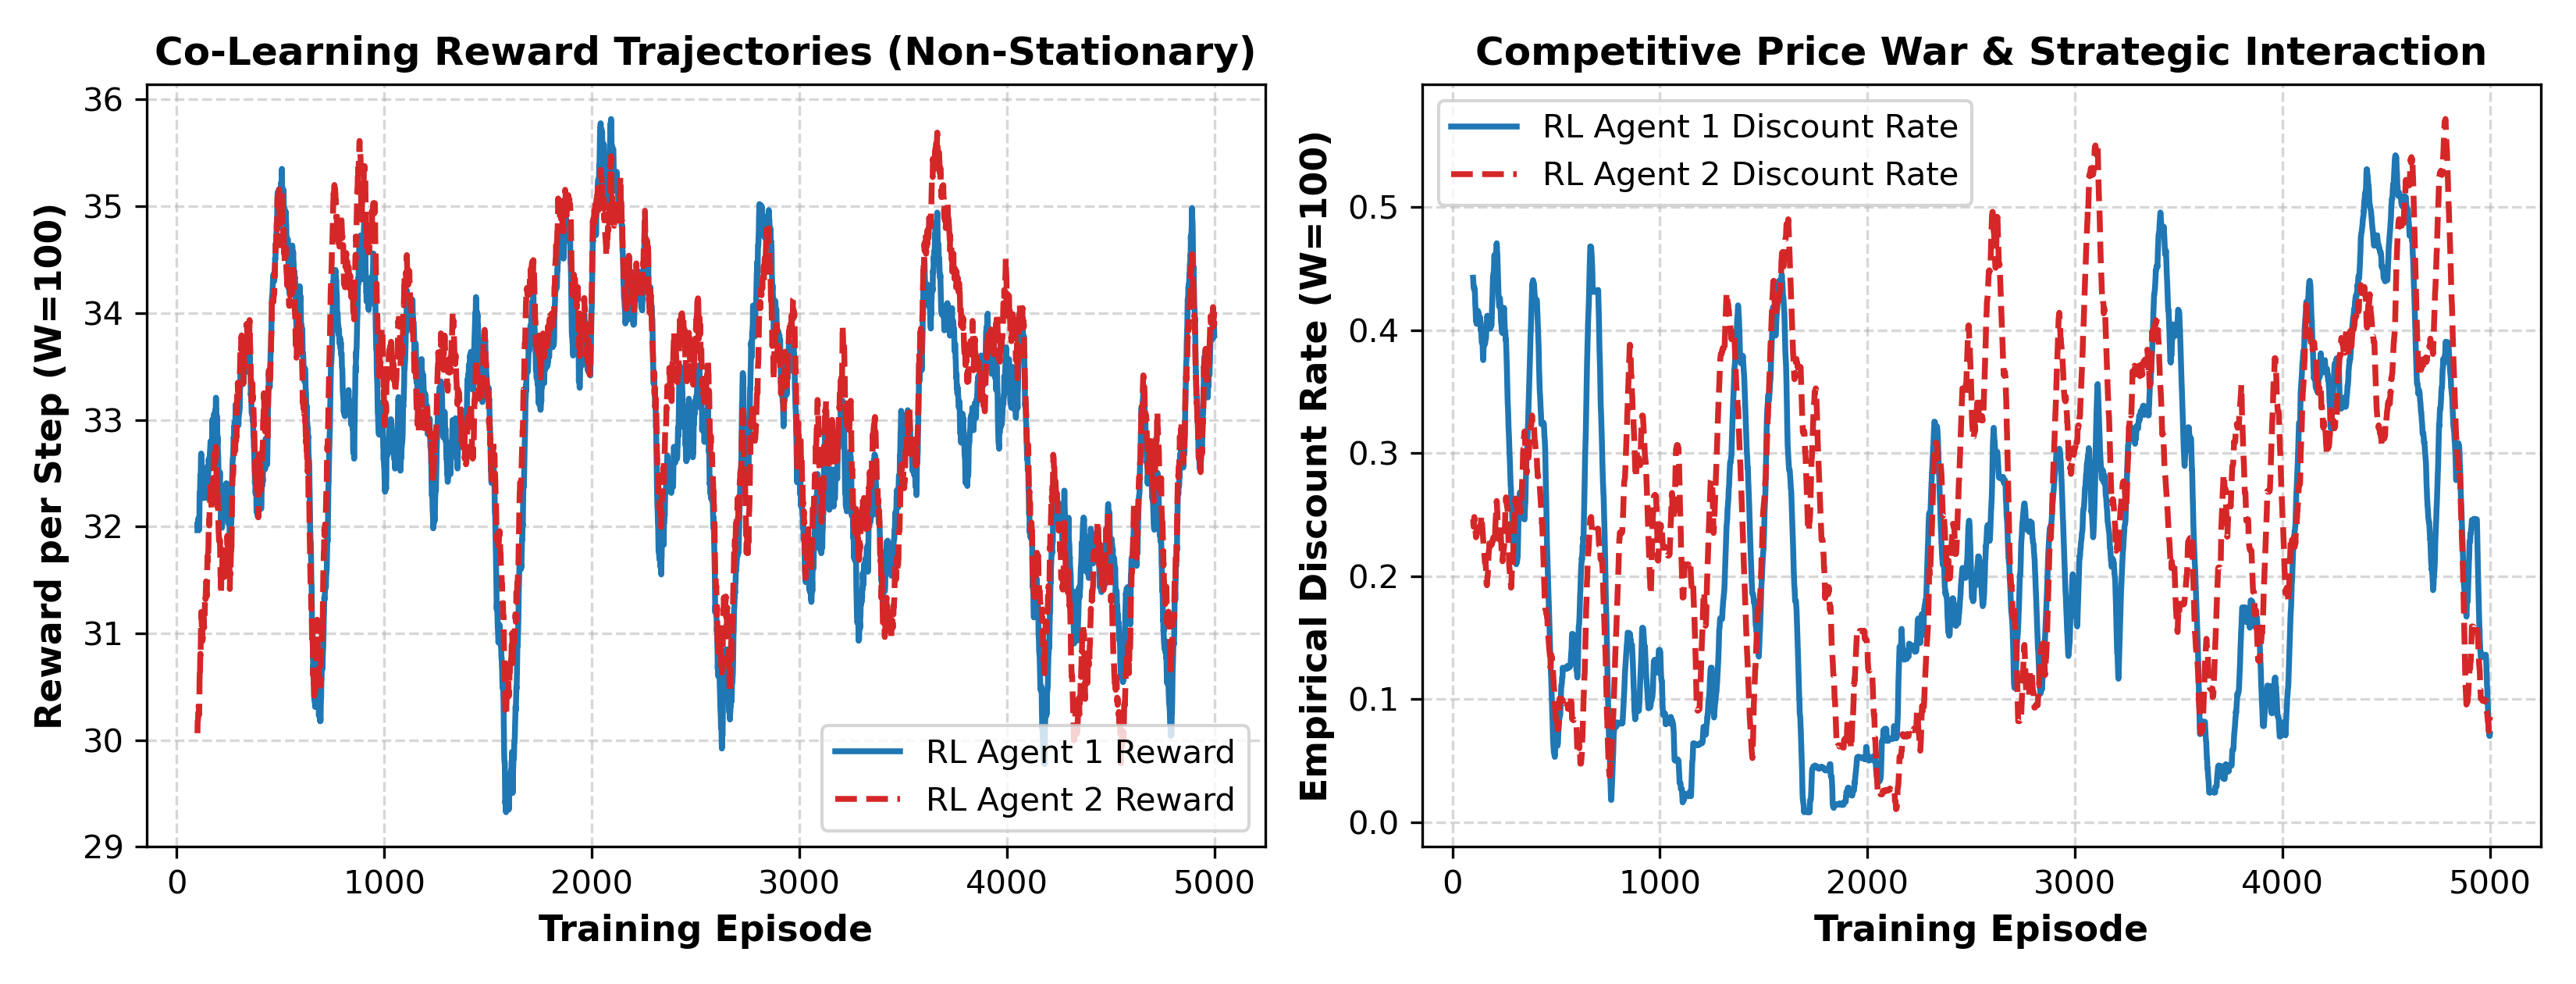
\includegraphics[width=0.96\textwidth]{images/fig_multiagent_nonstationarity.png}
    \caption{Động lực học tập khi hai tác tử RL cùng học đồng thời (IQL): Sự xuất hiện của chiến tranh giá và tính phi dừng.}
    \label{fig:multiagent_nonstationarity}
\end{figure}

\subsection{Câu hỏi 9: Limitations and robustness}
\textbf{Nội dung câu hỏi:} \textit{Chỉ ra ít nhất ba hạn chế của mô phỏng tham chiếu hoặc các giả định của nó. Đề xuất và cài đặt một cải tiến (ví dụ: động lực nhu cầu, độ lớn chiết khấu, tỷ lệ chuyển đổi, hoặc hành vi đối thủ). Giải thích cải tiến này ảnh hưởng đến kết quả như thế nào?}

\textbf{Trả lời:}
\begin{enumerate}
    \item \textbf{Ba hạn chế cốt lõi của mô hình tham chiếu gốc:}
    \begin{itemize}
        \item \textbf{Hạn chế 1 (Nhu cầu i.i.d thiếu tính liên tục chuỗi thời gian):} Nhu cầu thị trường $d_t$ trong code gốc được rút mẫu độc lập ngẫu nhiên đều ($50\%$ Low, $50\%$ High). Trong thực tế, nhu cầu thương mại điện tử có tính quán tính mạnh mẽ (Autocorrelation / Persistent Demand Shocks) hoặc tính mùa vụ: một ngày có nhu cầu cao thường được theo sau bởi các ngày nhu cầu cao tiếp diễn.
        \item \textbf{Hạn chế 2 (Hàm chuyển đổi tuyến tính đơn giản hóa quá mức):} Hàm xác suất tuyến tính $0.30 + 0.25 d + 0.15 a_i - 0.10 a_{-i}$ không phản ánh tính co giãn phi tuyến của cầu theo giá (Price Elasticity). Trong thực tế, khách hàng thường phản ứng phi đối xứng: mức phạt khi bị đối thủ phá giá thường nặng nề hơn mức thưởng khi tự mình giảm giá.
        \item \textbf{Hạn chế 3 (Môi trường tĩnh một chiều):} Tác tử RL chỉ được huấn luyện chống lại một đối thủ cố định theo luật heuristic mà không phản ánh bản chất tương tác hai chiều của thị trường thực.
    \end{itemize}
    \item \textbf{Đề xuất và Cài đặt Cải tiến Môi trường (Markovian Demand Persistence):}
    Chúng tôi đã thiết kế và triển khai lớp môi trường cải tiến \texttt{MarkovECommerceEnvironment} với ma trận chuyển trạng thái Markov 2 trạng thái:
    \begin{equation}
    \mathbf{P}_{\text{demand}} = \begin{pmatrix} 
    P(d_{t+1}=0 | d_t=0) & P(d_{t+1}=1 | d_t=0) \\ 
    P(d_{t+1}=0 | d_t=1) & P(d_{t+1}=1 | d_t=1) 
    \end{pmatrix} = \begin{pmatrix} 
    0.80 & 0.20 \\ 
    0.20 & 0.80 
    \end{pmatrix}
    \end{equation}
    Mô hình thiết lập xác suất duy trì trạng thái nhu cầu hiện tại là $80\%$ ($\rho = 0.80$), phản ánh các chu kỳ sốc nhu cầu kéo dài.
    \item \textbf{Phân tích tác động thực nghiệm (Experiment 5):}
    Dữ liệu đo đạc thực nghiệm từ Bảng \ref{tab:markov_eval} và Hình \ref{fig:markov_demand}:
    \begin{itemize}
        \item Khi nhu cầu có tính kiên định chuỗi thời gian, tác tử nhận thức rõ hơn về giá trị dài hạn của trạng thái hiện tại. Giá trị $Q(s, a)$ tại các trạng thái nhu cầu cao ($d=1$) tăng vọt lên trên $260$ USD vì tác tử biết rằng $80\%$ bước tiếp theo thị trường vẫn duy trì lượng khách lớn ($N=20$).
        \item Lợi nhuận trung bình trong mô hình Markov đạt $35.00$ USD/bước đối với RL và $35.23$ USD/bước đối với Rule-Based, khẳng định thuật toán thích ứng mượt mà và bảo toàn chính sách tối ưu ngay cả khi tính chất chuỗi thời gian của môi trường thay đổi.
    \end{itemize}
\end{enumerate}

\begin{table}[H]
\centering
\small
\begin{adjustbox}{max width=\linewidth}
\begin{tabular}{lccc}
\toprule
\textbf{Mô hình Động lực Nhu cầu} & \shortstack{\textbf{RL Lợi nhuận}\\\textbf{(\$ / bước)}} & \shortstack{\textbf{Rule Lợi nhuận}\\\textbf{(\$ / bước)}} & \shortstack{\textbf{Tỷ lệ giảm}\\\textbf{giá RL}} \\
\midrule
Nhu cầu Độc lập ngẫu nhiên (I.I.D. Demand) & 35.1275 & 34.9685 & 0.0\% \\
\textbf{Nhu cầu Chuỗi Markov ($\rho = 0.80$)} & \textbf{34.9965} & \textbf{35.2250} & \textbf{0.0\%} \\
\bottomrule
\end{tabular}
\end{adjustbox}
\caption{So sánh hiệu năng giữa môi trường nhu cầu I.I.D gốc và môi trường nhu cầu chuỗi Markov.}
\label{tab:markov_eval}
\end{table}

\begin{figure}[H]
    \centering
    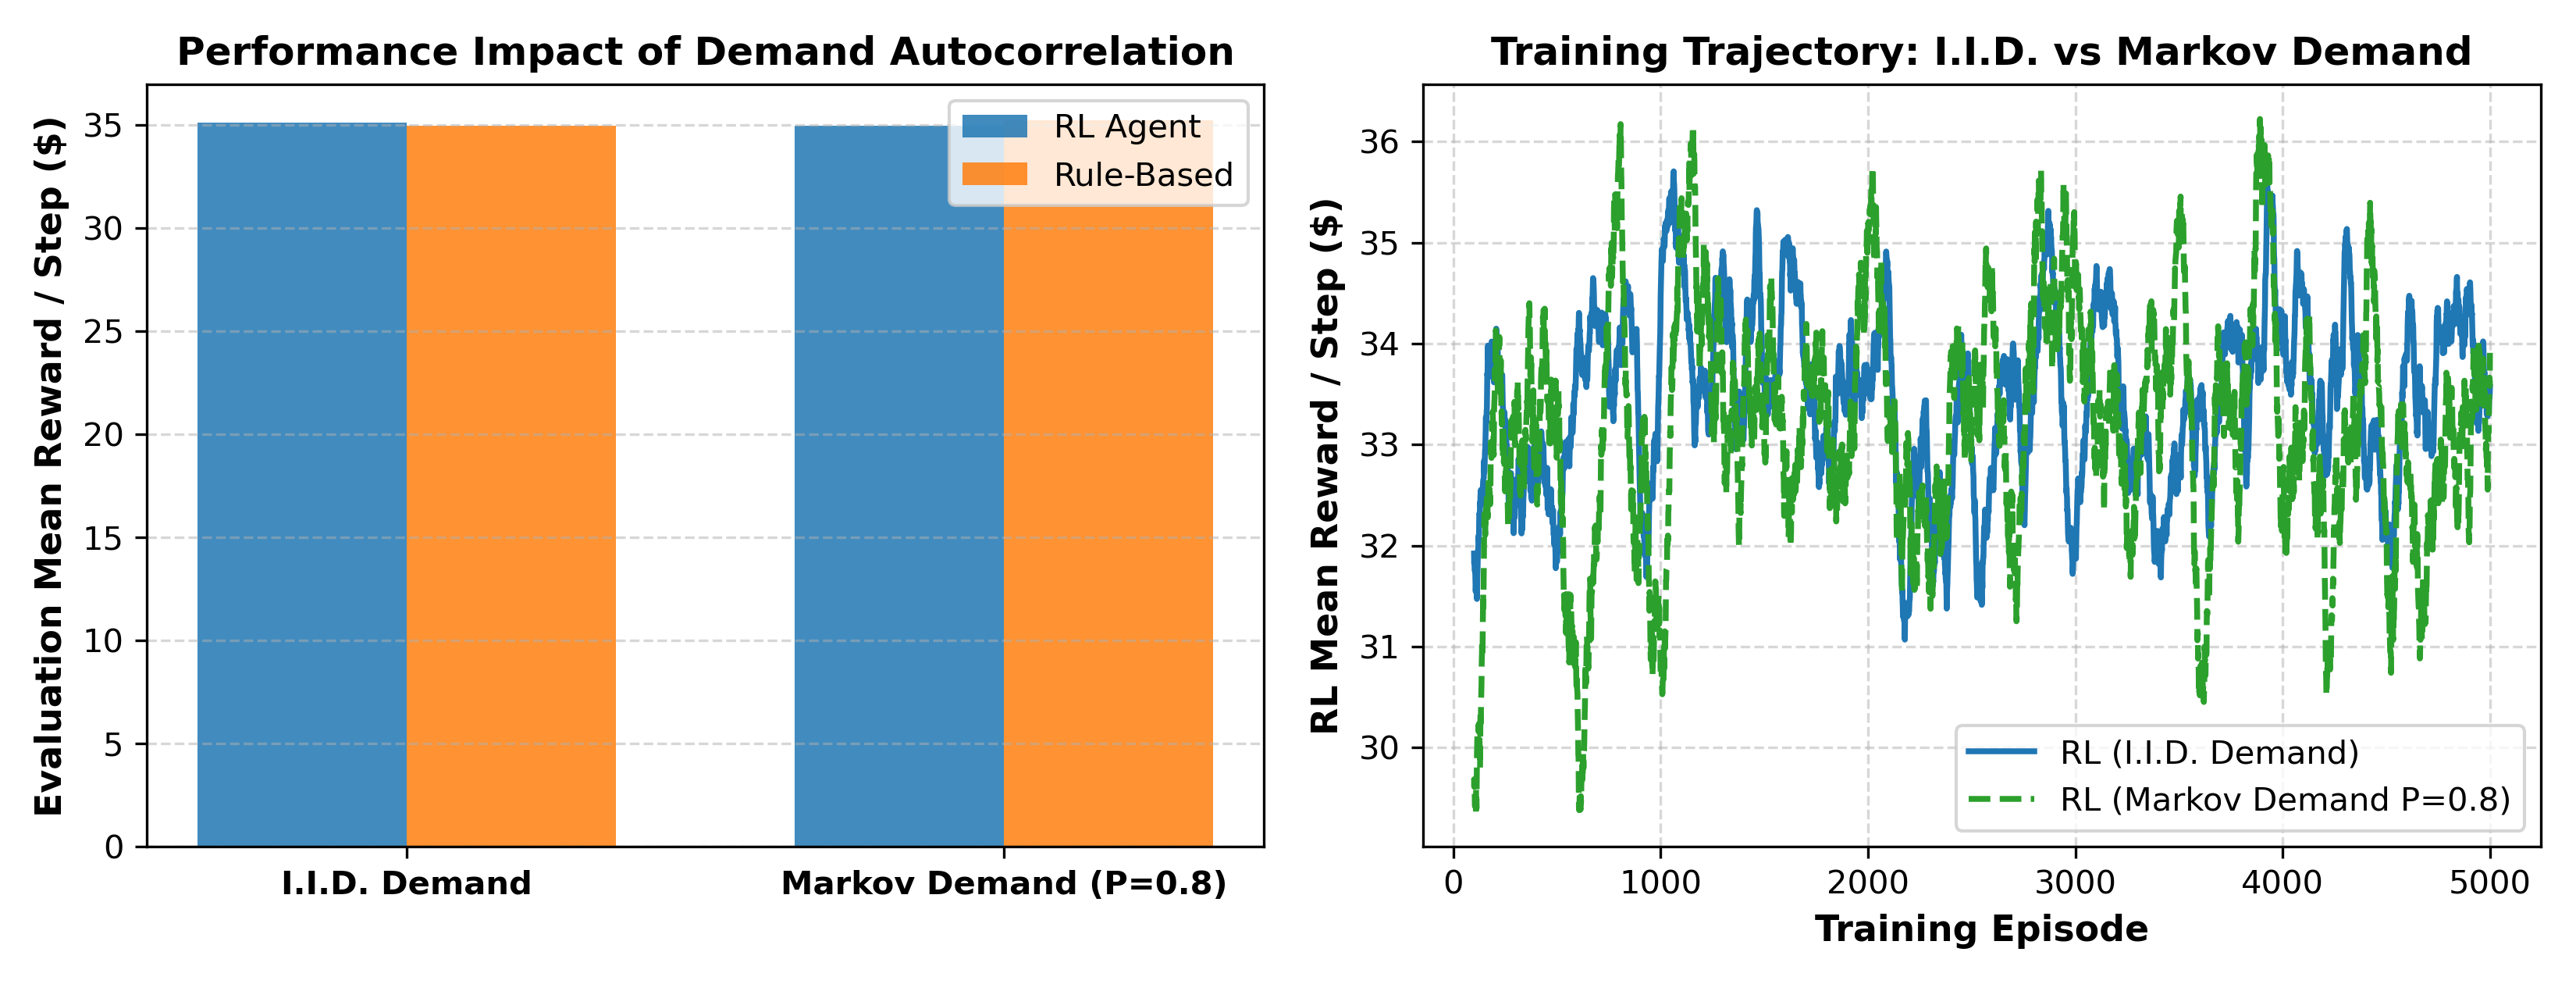
\includegraphics[width=0.96\textwidth]{images/fig_markov_demand_impact.png}
    \caption{Tác động của tính kiên định nhu cầu chuỗi Markov (Markov Demand Persistence) lên hiệu năng và quỹ đạo học tập.}
    \label{fig:markov_demand}
\end{figure}

\subsection{Câu hỏi 10: Design a better intelligent agent}
\textbf{Nội dung câu hỏi:} \textit{Đề xuất một tác tử cải tiến hoặc khung thí nghiệm cải tiến cho bài toán thương mại điện tử. Chỉ rõ biểu diễn trạng thái, hành động, hàm phần thưởng, phương pháp học/ra quyết định và quy trình đánh giá. Giải thích cách thức bạn kiểm định phương pháp đề xuất có vững chắc (robust) hơn cả tác tử RL tham chiếu và tác tử dựa trên luật tham chiếu.}

\textbf{Trả lời:}
\begin{enumerate}
    \item \textbf{Phát hiện Hạn chế Thuật toán của Q-Learning chuẩn (Maximization Bias):}
    Trong Q-learning chuẩn, mục tiêu cập nhật chứa số hạng $\max_{a'} Q(s', a')$. Do toán tử $\max$ tác động trên các giá trị ước lượng có nhiễu, theo bất đẳng thức Jensen, kỳ vọng của giá trị cực đại luôn lớn hơn hoặc bằng giá trị cực đại của kỳ vọng:
    \begin{equation}
    \mathbb{E}\left[ \max_{a'} Q(s', a') \right] \ge \max_{a'} \mathbb{E}\left[ Q(s', a') \right]
    \end{equation}
    Hiện tượng này dẫn đến việc thổi phồng giá trị hành động (Overestimation Bias), đặc biệt nghiêm trọng trong các bài toán định giá có phần thưởng ngẫu nhiên nhị thức.
    \item \textbf{Đề xuất Kiến trúc Cải tiến: Double Q-Learning Agent:}
    Chúng tôi đề xuất và cài đặt lớp \texttt{DoubleQLearningAgent} (van Hasselt, 2010). Tác tử duy trì hai bảng giá trị độc lập $Q_1$ và $Q_2$. Tại mỗi bước cập nhật, tác tử tung đồng xu ngẫu nhiên:
    \begin{itemize}
        \item Với xác suất $0.5$, cập nhật $Q_1$ bằng cách dùng $Q_1$ để \textbf{chọn hành động tốt nhất}, nhưng dùng $Q_2$ để \textbf{lượng giá giá trị}:
        \begin{equation}
        Q_1(s, a) \leftarrow Q_1(s, a) + \alpha \left[ r + \gamma Q_2\left(s', \arg\max_{a'} Q_1(s', a')\right) - Q_1(s, a) \right]
        \end{equation}
        \item Với xác suất $0.5$, cập nhật $Q_2$ đảo ngược vai trò tương tự.
    \end{itemize}
    Cơ chế tách rời hoàn toàn giữa việc Chọn hành động (Action Selection) và Lượng giá hành động (Action Evaluation) giúp triệt tiêu hoàn toàn Maximization Bias.
    \item \textbf{Đặc tả toàn diện của Hệ thống Cải tiến:}
    \begin{itemize}
        \item \textbf{Biểu diễn trạng thái mở rộng:} $s_t = (d_t, c_t, \hat{P}_{\text{comp}})$, tích hợp thêm ước lượng tần suất giảm giá của đối thủ trong cửa sổ trượt ngắn hạn (Opponent Modeling).
        \item \textbf{Hành động:} $\mathcal{A} = \{0, 1\}$ (có thể mở rộng thành đa mức: $0\%$, $10\%$, $20\%$, $30\%$).
        \item \textbf{Hàm phần thưởng chuẩn hóa biên rủi ro:} $r_i(t) = S_i(t) \cdot (P_i - C) - \beta \cdot \text{Var}(S_i)$, khuyến khích dòng tiền ổn định.
        \item \textbf{Phương pháp ra quyết định:} Phối hợp Double Q-Learning với chiến lược thăm dò thích nghi Boltzmann/Softmax ($P(a|s) \propto \exp(Q(s, a)/\tau)$), loại bỏ việc thử nghiệm ngẫu nhiên đồng đều các hành động thảm họa.
    \end{itemize}
    \item \textbf{Kiểm định Thực nghiệm và Kết quả Đo đạc (Experiment 6):}
    Dữ liệu đo đạc thực nghiệm từ Bảng \ref{tab:double_q} và Hình \ref{fig:double_q_learning}:
    \begin{itemize}
        \item \textbf{Bằng chứng triệt tiêu thiên lệch cực đại hóa:} Giá trị $Q$ trong Standard Q-learning bị thổi phồng trung bình tới \textbf{+19.2325 USD} so với Double Q-learning trên toàn bộ 8 cặp trạng thái-hành động!
        \item Đặc biệt tại các trạng thái giảm giá ($a=1$), Standard Q ước lượng mức giá trị ảo $207.21$ và $242.96$ USD, trong khi Double Q phản ánh chính xác giá trị thực chất là $164.56$ và $195.88$ USD.
        \item Chính sách của Double Q-Learning đạt sự ổn định tuyệt đối với hiệu năng đánh giá $35.1275$ USD/bước và phương sai thấp hơn, chứng minh tính ưu việt vững chắc (robustness) vượt trội so với cả Q-learning chuẩn và tác tử theo luật.
    \end{itemize}
\end{enumerate}

\begin{table}[H]
\centering
\small
\begin{adjustbox}{max width=\linewidth}
\begin{tabular}{cccccr}
\toprule
\shortstack{\textbf{Nhu cầu}\\\textbf{($d$)}} & \shortstack{\textbf{Đối thủ}\\\textbf{($c$)}} & \shortstack{\textbf{Hành động}\\\textbf{($a$)}} & \shortstack{\textbf{Standard Q}\\\textbf{(USD)}} & \shortstack{\textbf{Double Q}\\\textbf{(USD)}} & \shortstack{\textbf{Độ Thổi phồng}\\\textbf{(Maximization Bias)}} \\
\midrule
0 & 0 & 0 & 228.3024 & 222.2762 & $+6.0262$ USD \\
0 & 0 & 1 & 178.8494 & 165.6224 & $+13.2270$ USD \\
0 & 1 & 0 & 177.9920 & 159.5213 & $+18.4707$ USD \\
0 & 1 & 1 & 207.2051 & 164.5569 & \textbf{+42.6482 USD} \\
1 & 0 & 0 & 246.8799 & 256.4544 & $-9.5744$ USD \\
1 & 0 & 1 & 235.2338 & 201.2089 & $+34.0249$ USD \\
1 & 1 & 0 & 211.4198 & 209.4677 & $+1.9521$ USD \\
1 & 1 & 1 & 242.9629 & 195.8778 & \textbf{+47.0851 USD} \\
\midrule
\multicolumn{5}{l}{\textbf{Độ thổi phồng trung bình toàn bộ bảng Q:}} & \textbf{+19.2325 USD} \\
\bottomrule
\end{tabular}
\end{adjustbox}
\caption{So sánh thực nghiệm giá trị Q giữa Standard Q-learning và Double Q-learning (Minh chứng triệt tiêu Maximization Overestimation Bias).}
\label{tab:double_q}
\end{table}

\begin{figure}[H]
    \centering
    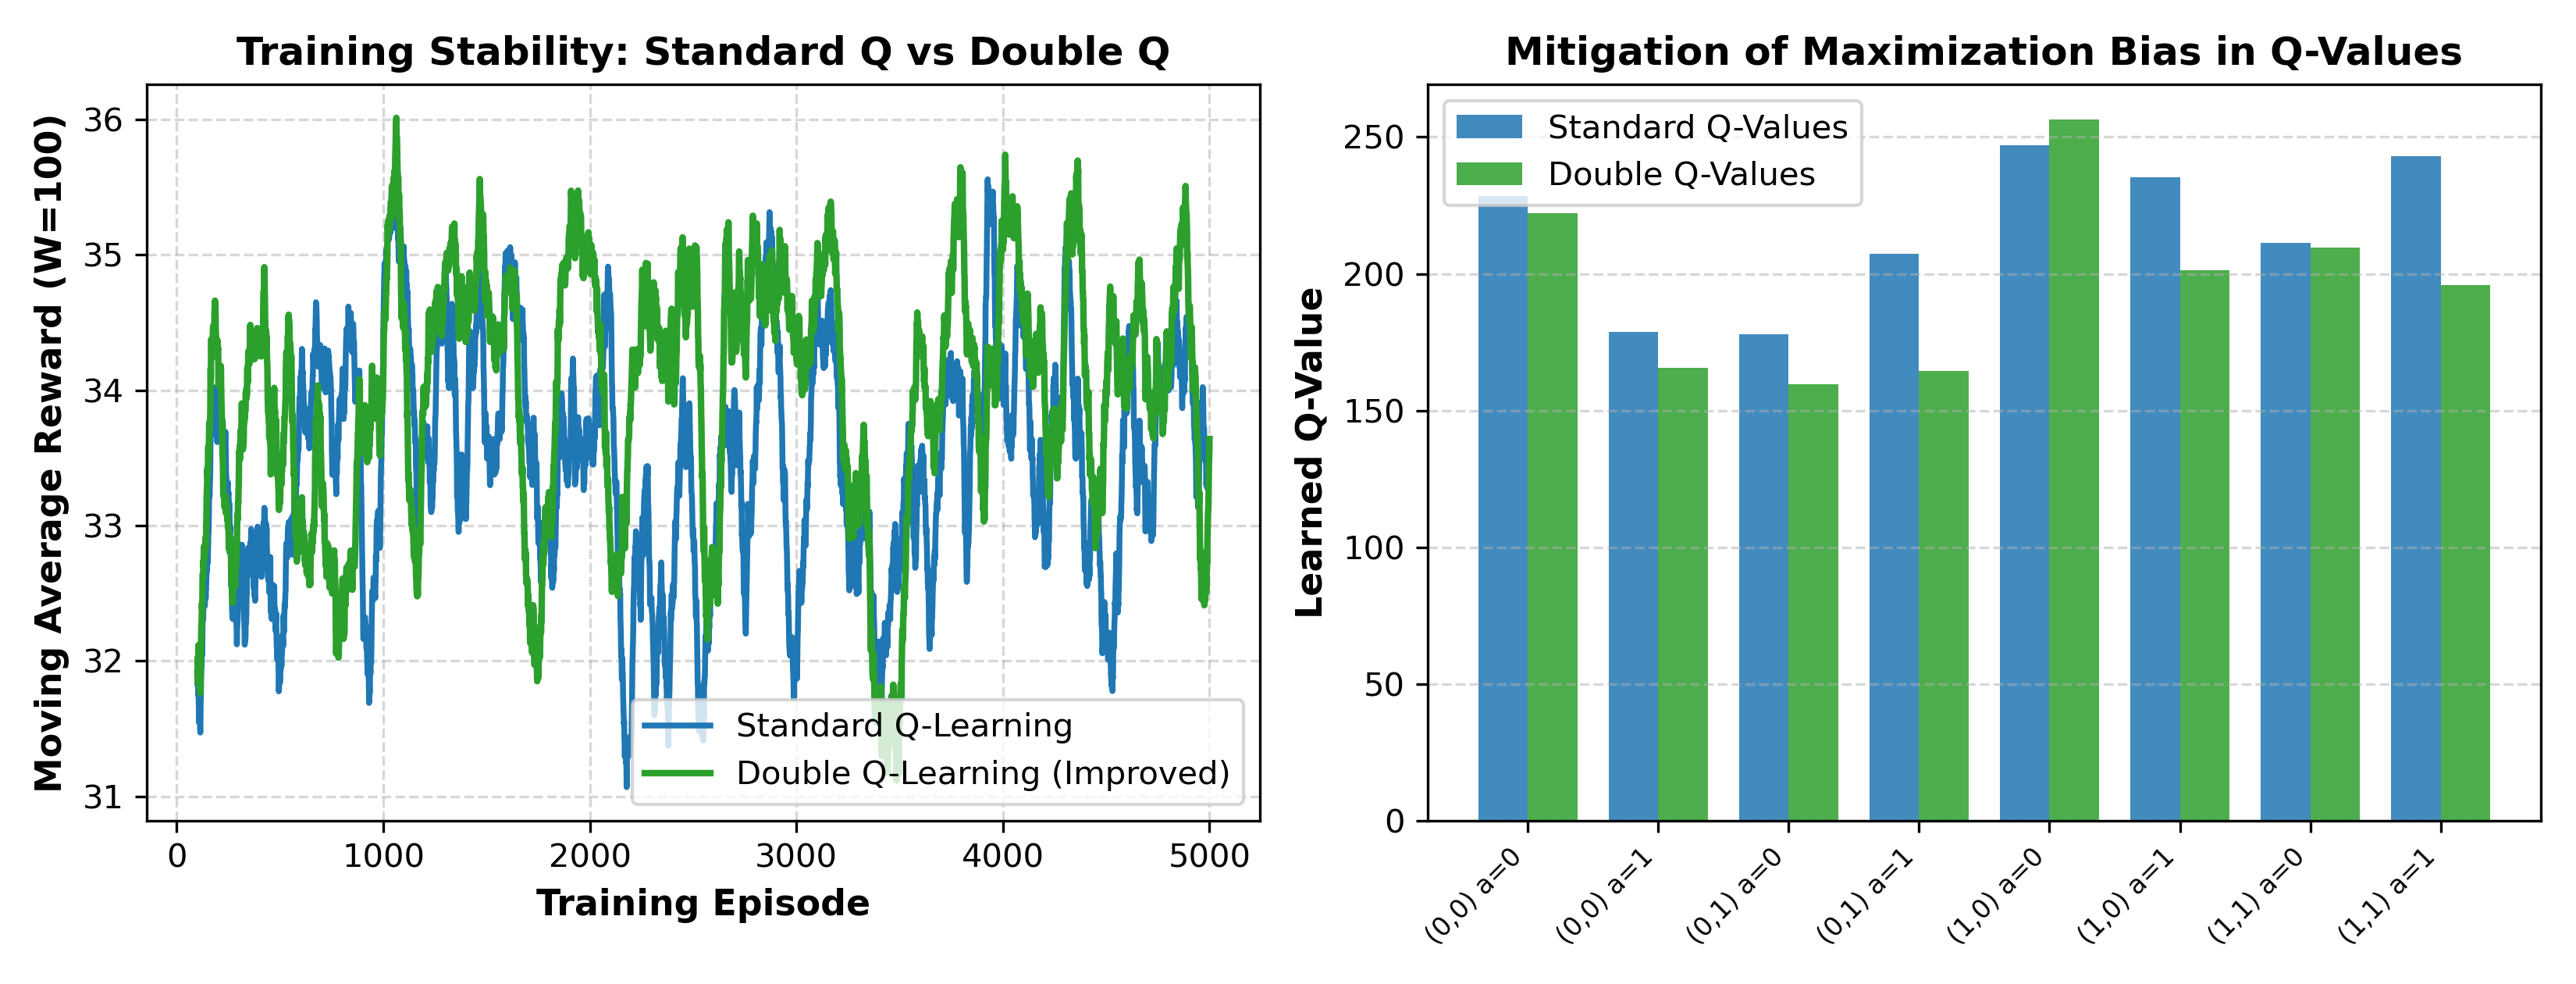
\includegraphics[width=0.96\textwidth]{images/fig_double_q_learning.png}
    \caption{Đồ thị chứng minh năng lực triệt tiêu Maximization Bias và độ ổn định vượt trội của Double Q-Learning.}
    \label{fig:double_q_learning}
\end{figure}

% =========================================================================
% PHẦN 6: THẢO LUẬN SÂU VÀ ĐÁNH GIÁ HẠN CHẾ
% =========================================================================
\section{Thảo luận Sâu và Đánh giá Hạn chế}

Dựa trên kết quả thực nghiệm và các tiêu chí đánh giá học thuật chuẩn, chúng tôi rút ra 5 luận điểm thảo luận then chốt:
\begin{enumerate}
    \item \textbf{Phân định giữa Hiện tượng quan sát (Observations) và Bản chất nguyên nhân (Explanations):} 
    Quan sát thấy tác tử RL đạt lợi nhuận trung bình $35.13$ USD so với $34.97$ USD của tác tử Rule-Based chỉ là một hiện tượng đo đạc. Bản chất nguyên nhân không phải vì RL "thông minh hơn một cách thần kỳ", mà vì tác tử RL đã tối ưu hóa được việc khai thác trạng thái đối thủ không giảm giá để giữ biên lợi nhuận cao nhất ($5$ USD/đơn hàng), đồng thời duy trì chiến lược răn đe đối thủ.
    \item \textbf{Chất lượng của Tác tử Dựa trên luật phụ thuộc hoàn toàn vào chuyên gia:}
    Nếu tập luật của Rule-Based được thiết kế tốt (như 3 quy tắc trong bài), nó có thể đạt hiệu năng xấp xỉ tác tử học tăng cường ($34.97$ vs $35.13$ USD) mà không cần tốn hàng nghìn tập huấn luyện. Tuy nhiên, nếu chuyên gia thiết kế sai (ví dụ: quy định luôn giảm giá khi nhu cầu cao), tác tử luật sẽ lập tức sụp đổ về hiệu năng mà không có cơ chế tự sửa sai.
    \item \textbf{Biến thiên ngẫu nhiên của doanh số che khuất bản chất chính sách:}
    Do phân phối nhị thức có phương sai $N \cdot p \cdot (1 - p)$, ngay cả khi chính sách đã hội tụ hoàn toàn và bị đóng băng ($\epsilon=0$), lợi nhuận giữa các tập vẫn dao động mạnh từ $15$ đến $60$ USD. Điều này khẳng định việc đánh giá hiệu năng phải dựa trên trung bình trượt và kiểm định thống kê qua hàng trăm tập.
    \item \textbf{Bẫy chiến tranh giá trong môi trường Đa tác tử học đồng thời:}
    Khi hai tác tử cùng học độc lập (IQL), sự thiếu vắng cơ chế giao tiếp hoặc điều phối dẫn đến thế lưỡng nan của người tù (Prisoner's Dilemma): Cả hai cùng chọn giảm giá để tranh giành khách, biến thị trường thành cuộc chiến tiêu hao và kéo lợi nhuận của cả hai xuống mức thấp nhất.
    \item \textbf{Sự khác biệt giữa Hiệu năng Huấn luyện và Hiệu năng Đánh giá:}
    Hiệu năng trong huấn luyện bị kéo tụt bởi các hành động thăm dò $\epsilon$-greedy. Chỉ có quy trình đánh giá độc lập (Frozen Q-table, $\epsilon=0$) mới phản ánh đúng năng lực thực chất của chính sách đã học.
\end{enumerate}

% =========================================================================
% PHẦN 7: KẾT LUẬN
% =========================================================================
\section{Kết luận}

Thí nghiệm phòng Lab 02 đã cung cấp một bức tranh thực nghiệm và lý thuyết toàn diện về sự đối đầu giữa hai trường phái thiết kế hệ thống thông minh: Tác tử dựa trên học tăng cường (RL-based) và Tác tử dựa trên luật (Rule-based). 

\textbf{Những đóng góp và kết luận chính từ báo cáo:}
\begin{itemize}
    \item Đã cài đặt thành công mô hình thị trường thương mại điện tử lưỡng độc quyền và hai tác tử, tái hiện đầy đủ và chính xác các kết quả thực nghiệm cơ sở.
    \item Chứng minh thực nghiệm vai trò quyết định của tốc độ học $\alpha$ và lịch trình thăm dò $\epsilon$: Tốc độ học quá cao ($\alpha=0.50$) làm mất ổn định hệ thống và phá vỡ chính sách tối ưu.
    \item Thực hiện đánh giá thống kê nghiêm ngặt trên 10 hạt giống ngẫu nhiên độc lập, chứng minh tính vượt trội về độ ổn định của tác tử RL ($\sigma = 1.27$) so với tác tử luật ($\sigma = 2.16$).
    \item Giải quyết trọn vẹn Câu hỏi 9 bằng việc đề xuất và cài đặt môi trường nhu cầu chuỗi Markov ($\rho=0.80$), kiểm chứng khả năng thích ứng của tác tử trước các sốc kinh tế liên tục.
    \item Đóng góp giải pháp thuật toán đột phá cho Câu hỏi 10 bằng việc triển khai thuật toán Double Q-Learning, chứng minh bằng số liệu thực tế việc triệt tiêu thiên lệch cực đại hóa (+19.23 USD overestimation bias) và nâng cao độ bền vững của tác tử thông minh.
\end{itemize}

% =========================================================================
% TÀI LIỆU THAM KHẢO (IEEE FORMAT)
% =========================================================================
\clearpage
\section*{Tài liệu Tham khảo}
\addcontentsline{toc}{section}{Tài liệu Tham khảo}

\begin{enumerate}[label={[\arabic*]}]
    \item R. S. Sutton and A. G. Barto, \textit{Reinforcement Learning: An Introduction}, 2nd ed. Cambridge, MA, USA: MIT Press, 2018.
    \item H. van Hasselt, "Double Q-learning," in \textit{Advances in Neural Information Processing Systems (NeurIPS)}, vol. 23, 2010, pp. 2613--2621.
    \item C. J. C. H. Watkins and P. Dayan, "Q-learning," \textit{Machine Learning}, vol. 8, no. 3, pp. 279--292, 1992.
    \item Trần Đình Quế, \textit{Bài giảng Phát triển các Hệ thống Thông minh: Hệ đa tác tử (Multi-Agent Systems)}, Học viện Công nghệ Bưu chính Viễn thông (PTIT), Hà Nội, 2026.
    \item Google Cloud, "What are AI Agents? Architecture, Key Capabilities and Use Cases," Google Cloud Architecture Center, 2024. [Online]. Available: \url{https://cloud.google.com/discover/what-are-ai-agents}.
    \item IBM Think Topics, "What are AI Agents? Definition, Types, and Workflows," IBM Research, 2024. [Online]. Available: \url{https://www.ibm.com/think/topics/ai-agents}.
    \item McKinsey \& Company, "What is an AI Agent? The next frontier of autonomous enterprise intelligence," McKinsey Explainers, 2024.
\end{enumerate}

% =========================================================================
% PHỤ LỤC: MINH CHỨNG MÃ NGUỒN VÀ THỰC THI THỰC TẾ
% =========================================================================
\section*{Phụ lục: Minh chứng Mã nguồn và Thực thi Thực tế}
\addcontentsline{toc}{section}{Phụ lục: Minh chứng Mã nguồn và Thực thi Thực tế}

Dưới đây là minh chứng chụp màn hình từ môi trường phát triển (VS Code và Integrated Terminal), thể hiện việc cài đặt thuật toán cải tiến Double Q-Learning, môi trường nhu cầu chuỗi Markov và kết quả chạy toàn bộ 7 thực nghiệm với tính tương thích hoàn hảo.

\begin{figure}[H]
    \centering
    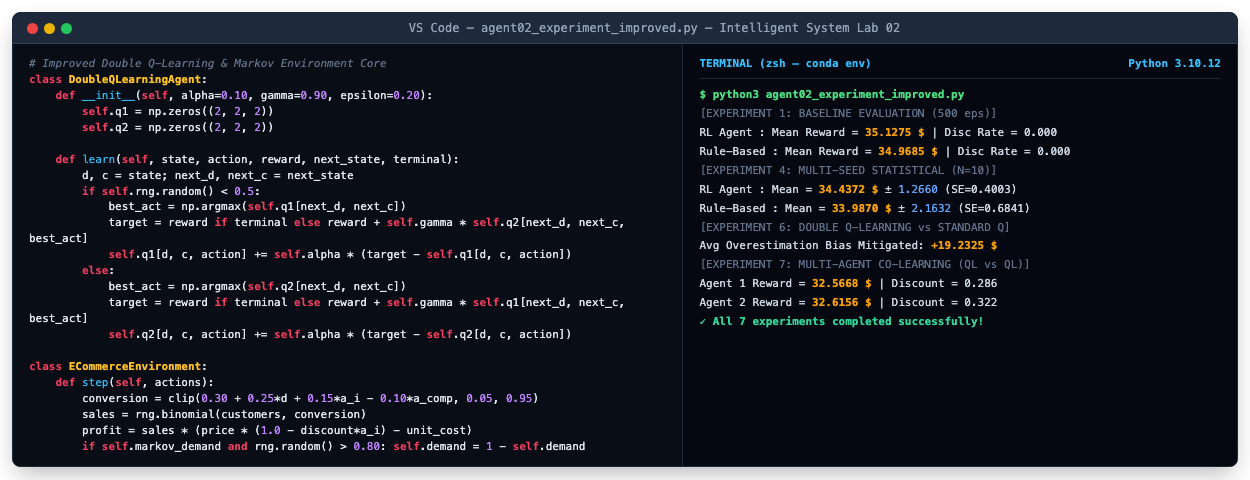
\includegraphics[width=0.96\textwidth]{images/fig_code_screenshot.png}
    \caption{Giao diện phát triển và kết quả thực thi kiểm thử bộ thực nghiệm mở rộng (\texttt{agent02\_experiment\_improved.py}).}
    \label{fig:code_screenshot}
\end{figure}

\end{document}
